%% Verze pro oboustranny tisk:
% Okraje: 
% (ale pozor, LaTeX si prida 1in)
\documentclass[10pt,a5paper,oneside]{book}
\usepackage[english,czech]{babel}
\usepackage[a5paper,margin=10mm]{geometry}
\newgeometry{top=20mm,bottom=20mm,right=15mm,left=15mm}
\usepackage{pdfpages}
\usepackage{textcomp}

\usepackage[utf8]{inputenc}

\usepackage[backend=bibtex, style=trad-unsrt]{biblatex}
\bibliography{DizertaceAutoreferat}

\DeclareBibliographyCategory{fullcited}
\newcommand{\mybibexclude}[1]{ \addtocategory{fullcited}{#1} }

\usepackage{url}
\usepackage[nottoc]{tocbibind}

%\usepackage{titlesec}  %vzhled titulku prvni stranky kapitoly
\selectlanguage{english}
\usepackage{fancyhdr}  %hlavicky stranek 

%% Ostatn� bal��ky
\usepackage{graphicx}
\usepackage{amsmath} % for mathematical equation
\usepackage{amssymb} % for special symbols - blacktriangledown
\usepackage[sc]{mathpazo} %palladio font
\usepackage[scaled]{helvet}
\usepackage{eulervm}

\usepackage{setspace} % for linespacing
\onehalfspacing 
\usepackage[T1]{fontenc} %font encoding e.g. for czech characters
\usepackage[intoc,refpage]{nomencl} % list of abbreviation

\makenomenclature
\renewcommand{\nomname}{List of Abbreviations}

%\usepackage{dtsyntax} % for listings modelica
%\usepackage[version=3]{mhchem} % for writing chemical compounds and reaction
%\usepackage{siunitx} % formating numbers
%\renewcommand{\ttdefault}{pcr} % nicer font - courier in listing

\usepackage[unicode,colorlinks]{hyperref}   % Musi byt za vsemi ostatnimi balicky
\hypersetup{pdftitle={Utilization of GRID in processing of medical information},
            pdfauthor={Tomáš Kulhánek},
            plainpages=false,
            urlcolor=blue,
            linkcolor=blue,
            citecolor=blue
            }

\makeatletter
\def\@makechapterhead#1{
  {\parindent \z@ \raggedright \normalfont
   \Huge\bfseries \thechapter. #1
   \par\nobreak
   \vskip 10\p@
}}
\def\@makeschapterhead#1{
  {\parindent \z@ \raggedright \normalfont
   \Huge\bfseries #1
   \par\nobreak
   \vskip 10\p@
}}
\makeatother

\begin{document}
\selectlanguage{english}

\shorthandoff{-} % fix problems with babel czech and includepdf chars '-' 
\pagenumbering{arabic} %first pages with roman numbering
\setcounter{page}{1}
\pagestyle{empty} % title page without number
\begin{center}
%\singlespacing 
\large
%\begin{tabular}{rl}
\textbf{\Large{Univerzita Karlova v Praze}}

\textbf{\Large{1.lékařská fakulta}} 

\textit{Charles University in Prague} 

\textit{1st Faculty of Medicine}
%\end{tabular}
\vfill
\normalsize
\begin{tabular}{rl}
Studijní obor:  & Biomedicínská informatika \\
\noalign{\vspace{-1mm}}
\textit{Study domain} & \textit{Biomedical informatics} \\
\end{tabular}

\vfill

{\Large Autoreferát dizertační práce}

\textit{\large Summary of the dissertation}

\vfill

\centerline{\mbox{
\includegraphics[width=40mm]{../img/logouk.png}

\includegraphics[width=40mm]{../img/logolf1.png}}}


\vfill



% N�zev pr�ce p�esn� podle zad�n�
\textbf{\large Využití technologie GRID při zpracování medicínské informace}

\vspace{2mm}
\textit{\large Utilization of GRID technology in processing of medical information}
\vfill
{\Large Mgr. Tomáš Kulhánek}

% N�zev katedry nebo �stavu, kde byla pr�ce ofici�ln� zad�na
% (dle Organiza�n� struktury MFF UK)
% CESNET z.s.p.o., Institute of pathological physiology



\vfill

Praha 2015

\end{center}


\pagestyle{plain} % other pages with number

\newpage
\selectlanguage{czech}
%\normalsize
\begin{center}
\textbf{Doktorské studijní programy v biomedicíně}

\textit{Univerzita Karlova v Praze a Akademie věd České republiky}
\end{center}
\normalsize

\vspace{2mm}

Obor: Biomedicínská informatika
\vfill
Předseda oborové rady: Prof. RNDr. Jana Zvárová, DrSc.
\vfill

Školicí pracoviště: CESNET z.s.p.o., Ústav patologické fyziologie 1.LFUK
\vfill


Školitel:  Ing. Milan Šárek, CSc.
\vfill

Konzultant:  Doc. MUDr. Jiří Kofránek, CSc. 
\vspace{100mm}

Disertační práce bude nejméně pět pracovních dnů před konáním obhajoby zveřejněna
k nahlížení veřejnosti v tištěné podobě na Oddělení pro vědeckou činnost a zahraniční styky
Děkanátu 1. lékařské fakulty.


\selectlanguage{english}

\setcounter{tocdepth}{0}
\tableofcontents
\newpage
\addcontentsline{toc}{chapter}{Abstrakt (česky)}

%%% Povinn� informa�n� strana diserta�n� pr�ce
\newpage
\begin{center}
\Large \textbf{Abstrakt (česky)}
\end{center} 
\normalsize
%\setlength\parindent{0mm}
%\setlength\parskip{2mm}
\selectlanguage{czech}
Práce se soustředí na vybrané oblasti biomedicínského výzkumu, které mohou profitovat ze současných výpočetních infrastruktur vybudovaných ve vědecké komunitě v evropském a světovém prostoru. Teorie výpočtu, paralelismu a distribuovaného počítání je stručně uvedena s ohledem na počítání v gridech a cloudech. Práce se zabývá oblastí výměny medicínských snímků a představuje propojení Gridového PACS systému s existujícími distribuovanými systémy pro sdílení DICOM snímků. Práce se dál zaměřuje na studium vědy týkající se lidského hlasu. Práce představuje vzdálený způsob přístupu k aplikaci pro analýzu hlasu v reálném čase pomocí úpravy protokolů pro vzdálenou plochu a pro přenos zvukových nahrávek. Tento dílčí výsledek ukazuje možnost využití stávajících aplikací na dálku specialisty na hlas. 

Oblast lidské fyziologie a patofyziologie byla studována pomocí přístupu tzv. systémové biologie. Práce přispívá v oblasti metodologie modelování lidské fyziologie pro tvorbu komplexních modelů založených na akauzálním a objektově orientovaném modelovacím přístupu. Metody pro studium parametrů byly představeny pomocí technologie počítání v gridech a v cloudech. Práce ukazuje, že proces identifikaci parametrů středně komplexních modelů kardiovasculárního systému a komplexního modelu lidské fyziologie lze významně zrychlit při použití cloud computingu a dobrých výsledků lze dosáhnout v rozumném čase. Tato metoda umožňuje aplikovat parametrické studie ve fyziologickém a biologickém výzkumu. Toto může zlepšit praktické použití matematických modelů a identifikaci parametrů ve zdravotní péči do budoucna.
%Technologie virtualizace zjedodušuje integraci doménově specifických aplikací do existujících výpočetních infrastruktur.


\textbf{Klíčová slova:}
gridové počítání, počítání v cloudu, výpočetní fyziologie, odhad parametrů, výměna medicínských snímků, analýza hlasového signálu


\addcontentsline{toc}{chapter}{Abstract}

\newpage
\begin{center}
\Large \textbf{Abstract}
\end{center} 

\normalsize
%\setlength\parindent{0mm}
%\setlength\parskip{2mm}
\selectlanguage{english}


This thesis focuses on selected areas of biomedical research in order to benefit from current computational infrastructures established in scientific community in european and global area. The theory of computation, parallelism and distributed computing, with focus on grid computing and cloud computing, is briefly introduced. Exchange of medical images was studied and a seamless integration of grid-based PACS system was established with the current distributed system in order to share DICOM medical images. Voice science was studied and access to real-time voice analysis application via remote desktop technology was introduced using customized protocol to transfer sound recording. This brings a possibility to access current legacy application remotely by voice specialists. 

The systems biology approach within domain of human physiology and pathophysiology was studied. Modeling methodology of human physiology was improved in order to build complex models based on acausal and object-oriented modeling techniques. Methods for conducting a parameter study (especially parameter estimation and parameter sweep) were introduced using grid computing and cloud computing technology. The identification of parameters gain substantial speedup by utilizing cloud computing deployment when performed on medium complex models of cardiovascular system and complex models of human physiology. This makes such kind of study applicable in order to perform identification of physiological system in reasonable time for physiological and biological research and good results are available in a reasonable time. This can improve practical usage of mathematical models in healthcare.

\textbf{Keywords:}
grid computing, cloud computing, computational physiology, systems biology, parameter estimation, medical image exchange, voice signal analysis



\clearpage
\markboth{\nomname}{\nomname}% maybe with \MakeUppercase
\printnomenclature
\clearpage
\pagestyle{fancyplain}
\fancyhf{}
\fancyhead[L]{ \fancyplain{}{\leftmark} }
\cfoot{ \thepage }

\selectlanguage{english}
\begingroup
\let\clearpage\relax

\section{Introduction}

The \emph{grid-computing} is usually defined as sharing computational and data storage resources across organizational boundaries. In recent years, the development of virtualization technologies enhances the availability of services provided by grid-computing and additionally enabled an evolution of so called \emph{cloud-computing}, which can utilize virtual environment on real powerful computing infrastructure too. Based on the development of technologies and also philosophy of providing them to end users, this thesis focus on multidisciplinary research related to grid-computing as well as to cloud-computing and it's utilization in biomedical research and application related to processing of medical information.

The term "medical information" is too wide and further work focuses on the following selected areas, which were part of:
(1) exchange and processing of medical images, (2) analysis of human voice and (3) modeling and simulation of human physiology. %This work focuses on processing of medical information should give enhanced information, which can be analysed easily. Thus further analysis or synthesis of such information is beyond this work, so the aim is not to give particular results on some specific diseasies, pathologies etc., however, with cooperation of other experts it is a desired side effect.

The author's work was published in a series of peer-reviewed papers of international journals and peer-reviewed conference proceedings \cite{kulhanek2009, kulhanek2010b, kulhanek2010c,  
Kulhanek2014Parameters, Kulhanek2014Modeling, Kulhanek2014mefanet, Matejak2014sj} which are attached into this work as appendices.
The author's work and contribution was also presented in international conferences and published in the respective proceedings and transactions
\cite{Kulhanek2010, Kulhanek2013c, kofranek2013hummod, Matejak2014}. The work was also popularized on the local and regional conferences and their respective proceedings \cite{Kulhanek2008Mefanet, Sarek2009, kulhanek2009dd, Kulhanek2009Mefanet, Kulhanek2010d, Kulhanek2010Mefanet, Kulhanek2011, kulhanek2011dd, Kulhanek2012, Kulhanek2013b, Kulhanek2014, Kulhanek2012a}. Author contributed to the utility model registered by the Czech Industrial Property Office \cite{Kofranek2014a}.

\section{Thesis Goal}
The hypothesis stated by this thesis is that the technologies related to grid-computing and cloud-computing may improve processing of medical information to perform demanding tasks which are almost impossible or may need onerous effort to achieve using classical local or institutional resources.
 
The aim of the thesis is to discuss the hypothesis in different areas of biomedical research and it's application.
The thesis tries to find answers to the following questions:
\begin{itemize}
\item \emph{What are the possible benefits and limitation of utilizing grid-computing (or cloud-computing) technology for processing medical information?} In the time of starting the work on this thesis, it was believed that grid-computing may be an answer to scalability issues of exchanging large ammount of data or doing demanding long-term computation. %In the field of medicine, such large ammount of data were exchanged using DICOM format and protocol explained in section \ref{sec:imaging} and the issue was to integrate it with computing infrastructure and tools designed for the purpose of science in particle physics.
%\item \emph{What are the limitation of utilizing these technologies?} In the time of starting the work on this thesis, the majority of services and tools in grid-computing environment were developed for the purpose of computation of particle physics experiments, however, infrastructure were designed to be open for any scientific domain.
\item \emph{What additional service should provide grid-computing or cloud-computing infrastructure?} In the time of starting the work on this thesis, the grid-computing infrastructure was used mainly to store, exchange and process medical data, mainly images in DICOM format and protocol (details in section \ref{sec:imaging}.
\item \emph{How should be designed the architecture of such services?} The main type of service design was service oriented architecture (SOA), while a focus was again get to plain old data objects represented e.g. in JSON format and processed by RESTful web services following REST architectural constraints (explained more in section \ref{sec:introintegration}.     
%\item	 Study the latest achievements in the field of exchanging medical images and study possible improvements using the grid-computing and cloud-computing technology.
%\item Analysis and processing of voice signal to support clinical and educational applications.
%\item analysis and mathematical modeling and simulation of biological systems
%\item Identify use cases in other fields of biomedicine which are suitable to utilize the power of grid-computing and cloud-computing infrastructure.
%\item Develop and test prototype application utilizing grid or cloud technologies.
\end{itemize}

\section{Thesis Contribution}
The author claims that the following contribution was made to the state of the art of biomedical informatics related to grid-computing and cloud-computing.
\begin{itemize}
\item Proposal of grid infrastructure and pilot implementation of grid-based system of exchanging medical images integrated with existing distributed systems. The results were published as \cite{kulhanek2009} and popularized as \cite{Kulhanek2008Mefanet,Sarek2009,kulhanek2009dd}. The author of this thesis customized the existing results of Globus MEDICUS project and deployed a grid application in the servers networked via academic network CESNET and integrated with existing regional PACS system. 
\item Pilot implementation of more generic infrastructure as a service for the community within the biomedical research \cite{kulhanek2010c, kulhanek2011dd}. The author of this thesis proposed the idea to share the physical resources and to provide virtual environment for specific needs of particular use-cases. With development of virtualization techniques and cloud-computing technologies the pilot infrastructure were tested on examples of selected research projects.
\item Proposal of software architecture and implementation of web-based service for real-time remote analysis of human voice. The results were published as \cite{kulhanek2010b} and popularized as \cite{Kulhanek2010d, Kulhanek2012}. The author of this thesis contributed to the idea of utilizing interactive remote access to the computing environment. For this reason it was identified requirements and customized the existing network protocol to transfer voice signal losslessly. Other co-authors implemented the algorithms and application to analyse voice signal.
\item Improved methodology for modeling of complex physiological systems \cite{Kulhanek2014Modeling, Kulhanek2014mefanet, Matejak2014, kofranek2013hummod}. Author of this thesis contributed to the idea of building complex  mathematical models from the basic components and keep them in an understandable and maintainable form utilizing some known good practices (patterns) and prevent bad practices (antipatterns) known from object-oriented programming. Author advised and implemented several basic blocks and models of pulsatile cardiovascular system in Modelica language. The other co-authors implemented the library to model physiology using integrative approach and implemented the complex models integrating different domains together.
\item Design and implementation of system to estimate parameters of complex mathematical models to validate or calibrate models of human physiology published as \cite{Kulhanek2014Parameters} and gradual development of related technologies were published and popularized as \cite{Kulhanek2010, Kulhanek2013c, Kulhanek2011, Kulhanek2014}. Author of this thesis designed the architecture for distributed parameter estimation algorithm and implemented pilot deployment utilizing scientific cloud-computing infrastructure and integrated complex model simulation with numerical identification algorithms. Other co-authors implemented complex models of human physiology in Modelica language and tested several algorithms for parameter estimation.
\item Improved mathematical model of oxygen, carbon dioxide and hydrogen ion binding to Hemoglobin \cite{Matejak2014sj}. Author of this thesis implemented this model in Modelica and calibrated the parameters of the model. Other co-authors analysed and proposed new mathematical model based on basic physical and chemical laws and relation published in literature.
\item Simulation of complex models of human physiology as part of virtual simulator on portable and mobile devices utilizing cloud-computing \cite{Kulhanek2013c,Kulhanek2013b}. Author of this thesis contributed to the idea of hybrid architecture of web simulators - utilizing the infrastructure for parameter estimation to simulate complex model remotely and process/visualize the results locally. Other co-authors implemented complex models of human physiology and specified and implemented simulation scenarios for educational purposes.
\item Virtual patient simulator prototype registered as utility model by the Industrial Property Office in the Czech Republic \cite{Kofranek2014a}. Author contributed to the development of prototype virtual simulator within module of cooperation of multiple instances within virtual classroom. Other co-authors designed and implemented models of human physiology, clinically relevant educational scenarios and implemented 3D visualization of selected scenarios using game engine Unity 3D\footnote{\url{http://unity3d.com/} accessed March 2015}.
\end{itemize}

\section{Thesis Structure}
This thesis is interdisciplinar, therefore the following chapters will cover the topics not-only from technical and computer-science point of view, but touches some topics related to the medical science mainly human physiology and it's mathematical models and simulations.
The chapter \ref{sec:stateoftheart} provides an overview of the state of the art in the theory of computation, parallel computation, distributed computation and focus on task-parallelization in grid-computing and cloud-computing infrastructure. 

%The chapter \ref{sec:methods} describes general methods available for integrating different technologies and specific methods used to obtain further results. 

Introduction, particular methods and results to selected areas of biomedical application and research are introduced in chapter \ref{sec:imaging} for sharing medical images, in chapter \ref{sec:voice} about voice science and chapter \ref{sec:models} about computational physiology.

The chapter \ref{sec:results} summarizes general results obtained by the research methods in specific areas of biomedical research and applications. The chapter \ref{sec:conclusion} discuss achievements and answers hypothesis and questions stated at the beginning of the work and recommends further direction of the research effort.

The appendices contain the selected papers \cite{kulhanek2009,kulhanek2010b,kulhanek2010c,Kulhanek2014Parameters, Kulhanek2014Modeling, Kulhanek2014mefanet, Matejak2014sj} which are most relevant to the topic of this thesis and which were published in international peer-reviewed journals or in peer-reviewed conference proceedings:

\textbf{Appendix~\ref{app:processing}} is the paper \cite{kulhanek2009} \emph{Processing of Medical Images in Virtual Distributed Environment} published by ACM as part of the proceedings of the 2009 Euro American Conference on Telematics and Information Systems: New Opportunities to increase Digital Citizenship.

\textbf{Appendix~\ref{app:remote}} is the paper \cite{kulhanek2010b} \emph{Remote Analysis of Human Voice – Lossless Sound Recording Redirection} published in Analysis of Biomedical Signals and Images. Proceedings of 20th International EURASIP Conference (BIOSIGNAL).

%\textbf{Appendix~\ref{app:fromeducational}} is the paper \cite{Kulhanek2011} \emph{From Educational Models Towards Identification of Physiological Systems} published by Institute of Biostatistics and Analyses of Masary University in Brno, Czech Republic in the proceedings Mefanet Report 04, Efficient multimedia teaching tools in medical education.  

\textbf{Appendix~\ref{app:infrastructure}} is the paper \cite{kulhanek2010c} \emph{Infrastructure for data storage and computation in biomedical research} published by Euromise s.r.o. in the European Journal of Biomedical Informatics.

\textbf{Appendix~\ref{app:parameter}} is the paper \cite{Kulhanek2014Parameters} \emph{Parameter estimation of complex mathematical models of human physiology using remote simulation distributed in scientific cloud} published in the IEEE Xplore Digital Library as part of the proceedings of the 2014 IEEE-EMBS International Conference on Biomedical and Health Informatics.

\textbf{Appendix~\ref{app:modeling}} is the paper \cite{Kulhanek2014Modeling} \emph{Modeling of short-term mechanism of arterial pressure control in the cardiovascular system: Object-oriented and acausal approach} published by ELSEVIER in Computers in Biology and Medicine 2014, \textbf{IF(2013): 1.475}.

\textbf{Appendix~\ref{app:simplemodelsd}} is the paper \cite{Kulhanek2014mefanet} \emph{Simple models of the cardiovascular system for educational and research purposes} published in Mefanet Journal 2014.

\textbf{Appendix~\ref{app:adair}} is the paper \cite{Matejak2014sj} \emph{Adair-Based Hemoglobin Equilibrium with Oxygen, Carbon Dioxide and Hydrogen Ion Activity} published in Scandinavian Journal of Clinical and Laboratory Investigation 2014, \textbf{IF(2013): 2.009}.

 %intro
\chapter{Hypothesis}

The hypothesis of this thesis is that the technologies that relate to grid computing and cloud computing may improve the processing of medical information in order to perform demanding tasks that are almost impossible or require onerous effort to achieve, using classical local or institutional resources.

The particular goals of this thesis are:
\begin{itemize}
\item To study the latest achievements in the field of exchanging medical images and  possible improvements using the grid computing and cloud computing technology.
%\item Analysis and processing of voice signal to support clinical and educational applications.
%\item analysis and mathematical modeling and simulation of biological systems
\item To identify use cases in other fields of biomedicine which are suitable to utilizing the power of grid computing and cloud computing infrastructure.
\item To develop and test the prototype application that utilizes grid or cloud technologies.
\end{itemize}

This thesis tries to discuss the hypothesis in different areas of biomedical research and its application which were identified during the work. (1) the exchange and processing of medical images, (2) the analysis of human voice and (3) the modeling and simulation of human physiology.

It tries to find answers to the following additional questions:
\begin{itemize}
\item \emph{Is it beneficial to utilize grid computing and cloud computing technology for the processing of medical information and how do we do this?} %The goal was to identify use cases in several fields of biomedicine which are suitable to utilize the power of grid-computing and cloud-computing infrastructure. Develop and test prototype application and compare achievements.%In the field of medicine, such large ammount of data were exchanged using DICOM format and protocol explained in section \ref{sec:imaging} and the issue was to integrate it with computing infrastructure and tools designed for the purpose of science in particle physics.
%\item \emph{What are the limitation of utilizing these technologies?} In the time of starting the work on this thesis, the majority of services and tools in grid-computing environment were developed for the purpose of computation of particle physics experiments, however, infrastructure were designed to be open for any scientific domain.
\item \emph{What are the limitations of processing medical information in grid or cloud?} 
\item \emph{How can the grid computing and cloud computing influence the direction of biomedical research?} There was an idea that grid computing technology inspires the current architecture of distributed systems,  e.g., exchanging medical images, and influences the direction of information systems in hospitals. 
\end{itemize}

 %hypothesis
\chapter{Methods}

From a computer science (informatics) point of view, it is assumed that the processing of medical information is, in general, a computational problem, which is understood as a task that can be solved by a computer. An algorithm is a set of operations that is used to accomplish tasks and solve problems. 
The important features of an algorithm are effectivity (what is the time complexity of the algorithm regarding the size of input data) and scalability (how far can an algorithm benefit from parallel computing). Grid computing and cloud computing brings a technology that enables parallel computing in a large amount of shared computers, servers or cluster of servers introduces large speedup of computation and can decrease the time of computation substantially. However, problems solvable by algorithms with exponential time complexity (e.g. NP-hard or NP-complete\nomenclature{NP-complete}{Nondeterministig Polynomial - complete}) can't be addressed by any large scale infrastructure \cite{Garey1979}. Therefore, additional non-exact methods for such type of problems are used to obtain at least some solution including heuristic method (eliminate some steps or solution classes that seems to not go to optimal solution), randomization (pseudo random values are generated and statistical methods can be used to compute expected optimal value) and others. 

\section{Sharing Medical Images}
The DICOM standard\footnote{DICOM: \url{http://dicom.nema.org/} accessed January 2015}\nomenclature{DICOM}{Digital Imaging and Communication Protocol} was used as a joint protocol to integrate grid-based system Globus MEDICUS \cite{Erberich2006} with current production system MEDIMED for sharing medical images among different hospitals \cite{Slavicek2010}, which is based on common distributed system with central cluster. 
% which may suffer with single point of failure and bottleneck issues. 
Globus MEDICUS \cite{Erberich2006,Erberich2007} implements a DICOM Grid Interface Service (DGIS) and integrates the open-source PixelMed\texttrademark ~Java DICOM Toolkit\footnote{\url{http://www.pixelmed.com/} accessed February 2015} into a web service, communicating via the DICOM protocol. Furthermore, it forwards queries to the underlying services within Globus toolkit. The console application of the MEDIMED project can be interconnected via DICOM protocol with local Picture Archiving and Communication System (PACS)\nomenclature{PACS}{Picture Archiving and Communication System} and selected DICOM studies can be sent/retrieved to another institution connected to the MEDIMED project.




%The typical workflow of a medical image in a hospital is in Figure \ref{fig:pacs}. 
%\begin{figure}[ht]
%    \centering
%    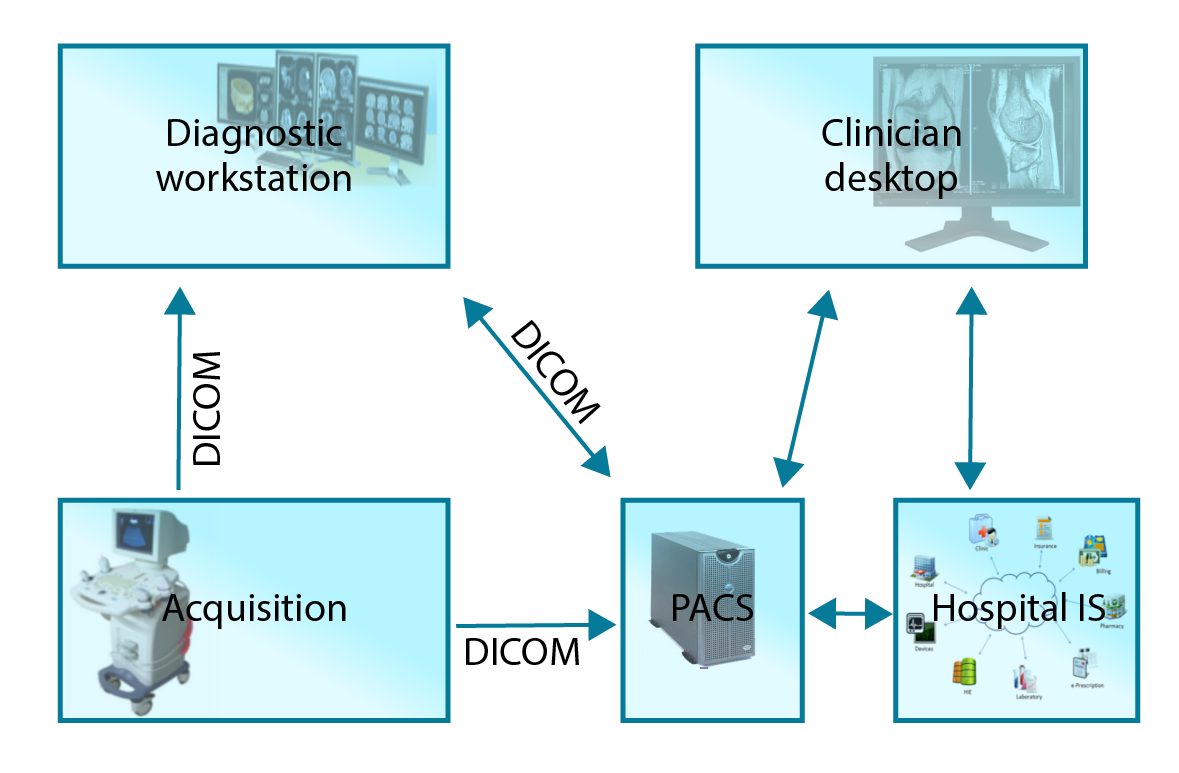
\includegraphics[width=0.7\textwidth, height=8cm]{img/chapter3-pacs.png}
%    \caption{Data acquisition is made by modalities (magnetic resonance, ultrasonography, etc.). By using the DICOM format and protocol, it can be directly transferred and visualized by diagnostic workstation. With the metadata filled by an expert physician, the image is stored in PACS. Other desktops within the hospital can retrieve the image and review the report.}
%    \label{fig:pacs}
%\end{figure}
%When there is need to share medical data records including medical images among different institutions and hospitals, a challenge should be solved with data confidentiality and size of the data. The DICOM\footnote{DICOM: \url{http://dicom.nema.org/} accessed January 2015}\nomenclature{DICOM}{Digital Imaging and Communication Protocol} standard is used for exchanging medical images electronically.  Picture Archiving and Communication System (PACS)\nomenclature{PACS}{Picture Archiving and Communication System} holds the acquired DICOM images with metadata and description, which are  noted by experts. PACS is usually part of the information systems in hospitals.
%
%

%\section{Sharing Medical Images}
%Various tools are already available within current grid infrastructures, including open-source and licensed software for computation. The local scientific grid provider may give a list of the available applications\footnote{applications available in CESNET METACENTRUM \url{https://wiki.metacentrum.cz/wiki/Kategorie:Applications} accessed February 2015}. Alternatively, application databases are available in a broader environment, e.g., in the EGI.eu application database\footnote{\url{https://appdb.egi.eu/} accessed February 2015}.
%Additionally, the workflow systems and scientific gateways that are mentioned in section \ref{sec:introworkflow} try to hide the complexity of grid or cloud computing infrastructures and may also be used to integrate specific domains.
%In designing a new application, the programming model of parallel computing and/or distributed  computing (in section \ref{sec:parallelprogramming} and  \ref{sec:distributedprogramming}) needs to be followed, utilizing the benefits of grid computing and cloud computing.

%The general approach to port applications to a grid infrastructure is to automatize what can be automatized, i.e., make scripts, configure system, prepare some user interface, integrate with existing applications, utilize protocol compatibility, etc. Additionally, the prepared template, script or application should be reused for further similar computational requests.

%\section{Sharing Medical Images}
%\label{sec:imaging}
%
%Use cases that relate to digital medical images involve image acquisition, preprocessing, storing and searching \cite{Bankman2000}.
%
%The acquisition of a medical image is performed with different modalities (different types of equipment and sensors) by radiologists or other specialists. The DICOM\footnote{DICOM: \url{http://dicom.nema.org/} accessed January 2015}\nomenclature{DICOM}{Digital Imaging and Communication Protocol} format and protocol has become an industrial standard for exchanging medical images electronically and in Picture Archiving Communication Systems (PACS). PACS holds the acquired DICOM images with metadata and description, which are  noted by experts. PACS is usually part of the information systems in hospitals. Figure \ref{fig:pacs} shows the typical workflows of a medical image in a hospital.
%
%
%
%%To summarize this section, in past years, 
%Digital medical image acquisition, storing, exchanging and processing has become common and it currently uses distributed computing techniques\cite{Slavicek2010, Ross2010, Saliba2012}. Several efforts have been made to implement medical data management within grid or cloud infrastructures for research purposes\cite{Erberich2006, Duque, Montagnat2007, Krefting2009, Krefting2010}  and to integrate them with production infrastructures \cite{Skaburskas2008, Benkner2010} or to share knowledge in semi-formally described semantics \cite{Kuba2006}.
%
%The Globus toolkit belongs to a group of the most used grid middleware (see section~\ref{sec:servicegrid}). 
%%The core service included in Globus Toolkit is GridFTP -- grid extension to file transfer protocol(FTP)\nomenclature{FTP}{File Transfer Protocol}. This implements strategies such as \emph{stripping data} into multiple pieces; the \emph{parallel transfer of data}, utilizing stripped data parts to be transferred via different channels; \emph{partial file transfer}, some applications may not need to access the whole file but rather a smaller portion of it, etc., as described by Foster et al. and Allcock et al. \cite{Foster2006, Allcock2005}. Other core services are Replica Location Service, which aims to localize data, and Globus Resource Allocation Management (GRAM), which provides web service and proxies to the lower level job scheduler's implementation \cite{Foster2006}.
%%Next to core services, the domain-specific services might be implemented for the purpose of an application that uses the Open Grid Service Architecture (OGSA). 
%Globus MEDICUS \cite{Erberich2006,Erberich2007} implements a DICOM Grid Interface Service (DGIS) and integrates the open-source PixelMed\texttrademark ~Java DICOM Toolkit\footnote{\url{http://www.pixelmed.com/} accessed February 2015} into a web service, communicating via the DICOM protocol. Furthermore, it forwards queries to the underlying services within Globus toolkit. 
%
%%DGIS acts as a gateway to a grid infrastructure. As communication via the DICOM protocol is not secured, it is recommended that the DGIS be installed on the location of the PACS system or the DICOM ready modality or software. When a DICOM study is uploaded into DGIS, it is anonymized and stored. A record is made into another service’s Meta Catalog service, which resides in the same domain or anywhere in the grid that is accessible via the Globus Toolkit. Such an anonymized database of DICOM records can be used to query via the DGIS interface and to, for example, integrate with web-based applications, showing records for research purposes. Furthermore, authentication and authorization can be achieved in this level. 
%To integrate this system with an existing system MEDIMED project \cite{Slavicek2010} for sharing the medical images, the special client software "RediMed console", needs to be installed next to the DGIS. DGIS behaves as an access point to a PACS system whose records can be exchanged via the RediMed console software to other MEDIMED participants. 
%The results of this particular deployment and integration are presented in section \ref{sec:resultsimages}.
%
\section{Voice Science}
\label{sec:voice}

The software for parameterized Voice Range Profile (ParVRP) and Voice Range Profile in Real time (RealVoiceLab) was already developed and calibrated for selected types of microphones in an MS Windows platform by Fric et al. \cite{Fric2007,Fric2012}. Its implementation is carried out in an MATLAB environment, utilizing Signal Processing Toolbox\footnote{\url{http://www.mathworks.com/products/signal/} accessed February 2015}. It is compiled with a MATLAB Compiler and distributed as an executable. To migrate this legacy application into distributed environment, the virtualization can be used with a protocol to control an application remotely. Remote Desktop Protocol (RDP)\nomenclature{RDP}{Remote Desktop Protocol} is a proprietary protocol that is used for desktop sharing. It was primarily developed in a Microsoft Windows platform, however, today, clients and servers exist for several other platforms. RDP itself contains the redirection of several services, e.g., audio, sound recording, drive access, etc. 

%With the introduction of objective data analysis and laryngoscopy methods, voice science emphasized the cooperation among laryngologists, speech pathologists and voice teachers.
%The normal human voice ranges from 50 Hz to about 1~000 Hz and there are some  individual variations. For the analysis of a digitally recorded voice, either habitual or singing, the Discrete Fourier Transformation (DFT)\nomenclature{DFT}{Discrete Fourier Transformation} is used to produce a frequency and amplitude analysis of the recorded input voice samples. One of the most used class algorithm to compute DFT is the class of Fast Fourier Transformation (FFT)\nomenclature{FFT}{Fast Fourier Transformation} with computational complexity $O(n \log(n))$ \cite{Cooley1965,Frigo2005}.
%% and parallel version of the algorithms may introduce additional speedup for larger samples of analyzed data \cite{Gupta1993,Takahashi2003}. 
%The result of the analysis can be visualized in a voice range profile (VRP)\nomenclature{VRP}{Voice Range Profile} (Figure \ref{fig:vrp} and the significant difference between an untrained and trained voice can be seen, as published, e.g., by LeBorgne and Weinrich showing a signficant difference of VRP after nine-month training \cite{DeLeoLeBorgne2002}. Furthermore, some disorders can be quantitatively seen, which were published, e.g., by Wuyts et al.\cite{wuyts2003effects}.
%\begin{figure}[ht]
%    \centering
%    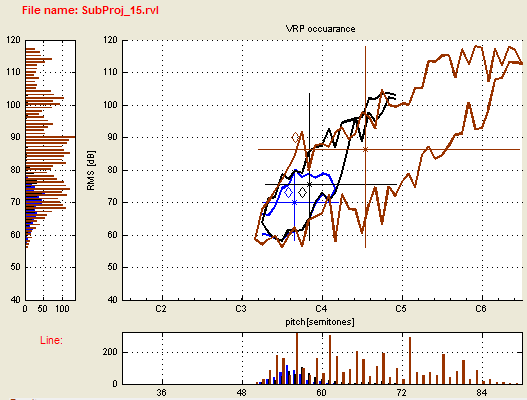
\includegraphics[width=0.8\textwidth, height=8cm]{img/autoreferat-vrp.png}
%    \caption{Voice Range Profile shows maximum and minimum intensity levels (y-axis) across the vocal range (x-axis) of normal speech (area surrounded by blue line) and singing (area surrounded by brown line).
%    }
%    \label{fig:vrp}
%\end{figure}
%
%%Another method that is used to analyze vocal chords is laryngoscopy. The videostroboscopy and high speed video in laryngoscope methods produce videos showing real movement of vocal chords. The videokymography method, introduced by Švec et al., complements the videostroboscopy. It allows the visualizing and analyzes of the movement of vocal cords. These movements are recorded by a high speed camera and an new image constructed from selected line of recorded video, which can be shown on standard TV or monitor using low frequency \cite{Svec1996,Svec2007}. 
%
%%In the case of a recorded sound and further analysis, there is a question about how such a service can be integrated in a grid computing or cloud computing environment in order to provide access to a complex application for non-technical voice specialists. Additionally, analytical software was already developed and calibrated for selected types of microphones in the MS Windows platform by Frič et al. \cite{Fric2007,Fric2012}. Therefore, I proposed and implemented a method that provides remote access to the analytical software. Section \ref{sec:methodsvoice} describes how the analytical software was customized with a remote desktop protocol (RDP)\nomenclature{RDP}{Remote Desktop Protocol}. Results are described in section \ref{sec:resultsvoice}. A similar approach can be used for processing  video recordings from a laryngoscope, however, the practical limits are discussed in section \ref{sec:conclusion}. 
%
%%\subsection{Methods for Remote Analysis of the Human Voice}
%\label{sec:methodsvoice}
%Terminal access to some remote computational capabilities, e.g., remote command-line or remote execution, is another integration strategy that is used for some remote infrastructures. Secure Shell (SSH) is used to establish a secure channel via an unsecured network (e.g., the Internet) from an SSH client to a SSH server. This is a basic method that is used to access a grid computing infrastructure. 
%Remote Desktop Protocol (RDP)\nomenclature{RDP}{Remote Desktop Protocol} is a proprietary protocol that is used for desktop sharing. It was primarily developed in a Microsoft Windows platform, however, today, clients and servers exist for several other platforms. Next to remote command-line, remote execution allows the accessing of remote graphical desktop environments. 

%
%%The computation of frequencies and amplitude from the recorded samples utilizes the effective Fast Fourier Transformation, which has time complexity $O(n\log(n))$. The benefit of deploying such an application in distributed infrastructures is the immediate access to updated software. Additionally, a collection of anonymized records of voice samples and results are very useful for further research and education. The possible disadvantage is the need to access to Internet.
%
%%This type of application can be packaged as a virtual machine template and configured within different types of cloud infrastructures. Together with a script or web portal, the on-demand deployment can be automated. The client part (RDP client) needs to connect to the appropriate instance. The results of such a deployment are discussed in section~\ref{sec:resultsvoice}.
%
\section{Computational physiology}
\label{sec:models}
A mathematical formalization of the fundamental knowledge and relation among a biological system – a mathematical model - is used as a base abstraction in order to utilize the current discoveries of the genomics and proteomics. It is also used to formalize the knowledge and construct a "Physiome Model". By  definition, a model is the simplification of a complex reality. Constructing the models and integrating them into a complex entity, which can be used for further purposes, is schematically illustrated in Figure \ref{fig:modeling}. 

\begin{figure}[ht]
    \centering
    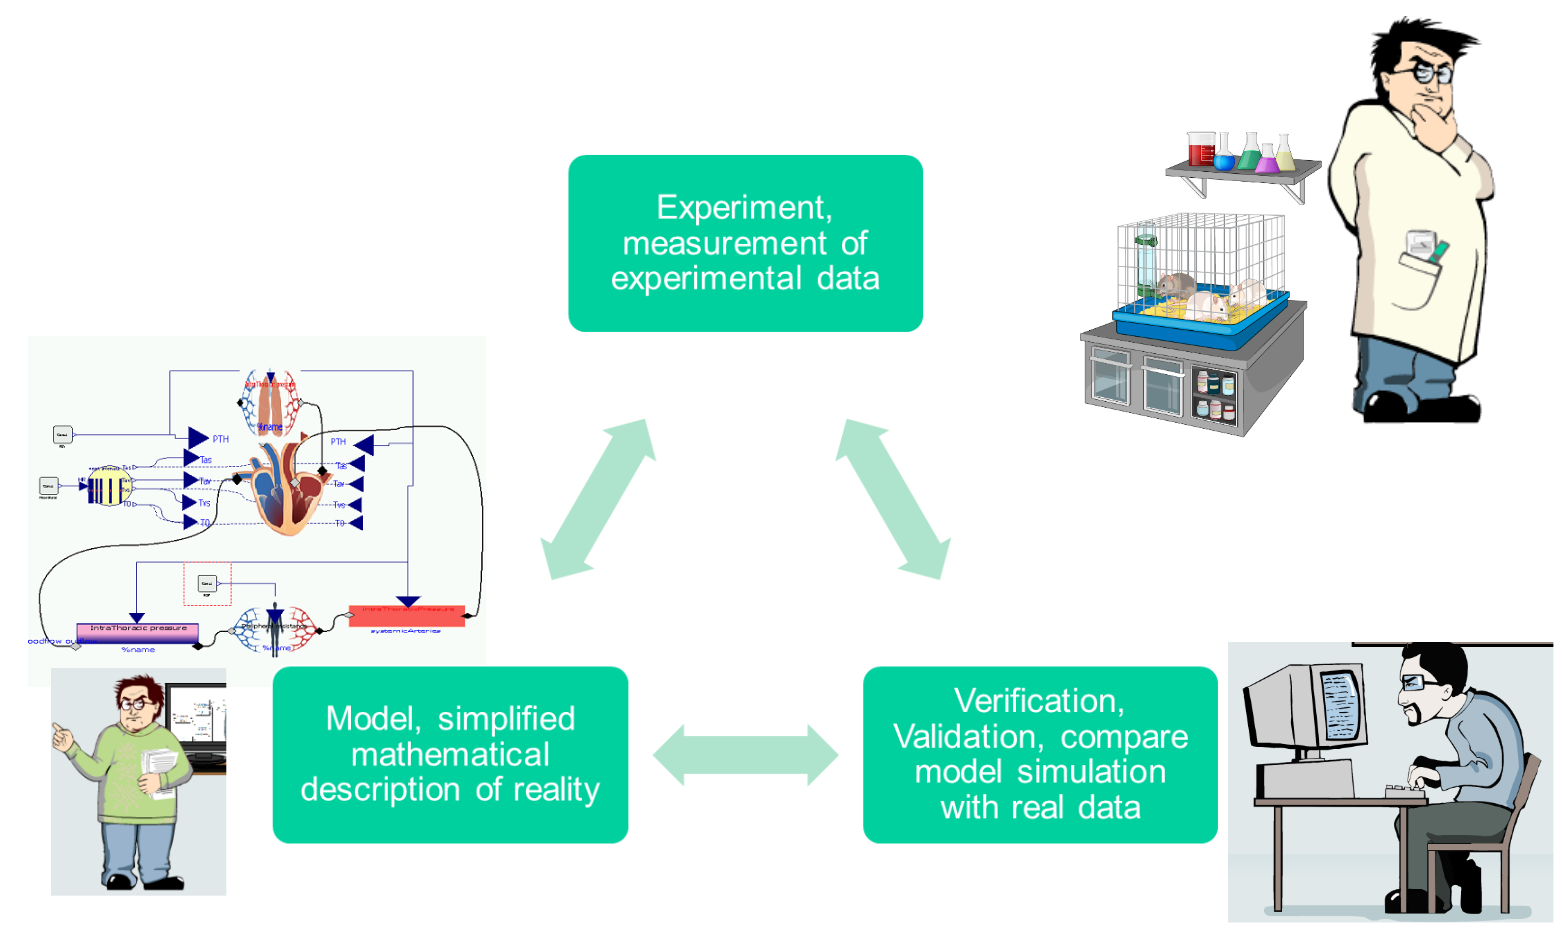
\includegraphics[width=1\textwidth]{../chapter3/modeling.png}
    \caption{Schematic illustration of the scientific process. The experiments produce data that are interpreted and a hypothesis is formalized as a model. Validation compares the model simulation with the experiment, if the model satisfies the criteria -- if it is in agreement with real experiments -- then the validated model can be used for other purposes. 
    }
    \label{fig:modeling}
\end{figure}

There are used several technologies in order to implement a formalized model of physiology. Within the work of this thesis a Modelica language was choosen, because it was identified as robust to maintain most complex models of human physiology in understandable way \cite{Kofranek2011hummod}. Additionally, a library Physiolibrary developed by Matejak et al. (21.) %\cite{Matejak2014} 
was enhanced and used especially within the hydraulic domain components as listed in Table \ref{table:physiolibrary}. 

\begin{table}[!ht]
\small
\centering
\begin{tabular}{m{1.0cm} m{10.2cm}}
%\begin{tabular}{m{1.2cm} m{13.5cm}}
\hline
Icon & Description \\
\hline
%\begin{tabular}{m{1.5cm} m{12.7cm}}

\includegraphics[scale=0.8]{HydraulicPorts.png} & Acausal hydraulic connectors -- the MODELICA tool generates "Kirchhoff law" analogy for all non-flow variables $p_1 .. p_n$ (pressure) and "flow" variable $q1..q_n$ (flowrate):\\
 & $ \label{eq:con1} p_1 = p_2 =... = p_n$ \\
 & $ \label{eq:con2} \sum_{i=1}^{n} q_i = 0$  \\
\hline
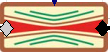
\includegraphics[scale=0.4]{resistance.png} & Hydraulic Resistor--characterized by $G$--conductance parameter (reciprocal value of resistance $G = 1/R$) and defined by relation among quantities from both hydraulic connectors, $q$--flowrate and $(p_{out} - p_{in})$ --pressure gradient:\\ 
 & $ \label{eq:resistor} q = G *(p_{out} - p_{in}) $ \\ \hline

\includegraphics[scale=0.4]{elasticity.png} & Elastic compartment--characterized by parameters: $C$--compliance (reciprocal value of elastance $C=1/E$), $V_0$--unstressed volume, $p_0$--external pressure. The relation among $p$--pressure, $V$--volume and $q$--flowrate are:\\ 
& $ \label{eq:compliance}p-p_0 = \left\{   
  \begin{array}{l l} 0 & \quad \text{if } V \text{\textless} V_0 \\ 
    \frac{V-V_0}{C} & \quad \text{otherwise}
  \end{array} \right.$ \\
 & $ \label{eq:flowrate}\frac{{\rm d}V}{{\rm d}t} =  q$ \\ 
 \hline
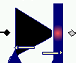
\includegraphics[scale=0.5]{valve.png} & Valve is characterized by $g_on$ -- inflow, $g_off$ -- backflow conductance and $P_{knee}$ forward threshold pressure. The relation for $dp$ pressure gradient and $q$ flowrate between the two connectors are:\\
 & $dp = \left\{ \begin{array}{lr} pass/g_{on} +P_{knee} & \text{for } pass >0 \\
   pass + P_{knee} & \text{otherwise} \end{array} \right. $ \\
% & $dp = \left\{ \begin{array}{1 1} pass/g_{on} +P_{knee} & \text{for } pass >0 \\
%   pass + P_{knee} & \text{otherwise} \end{array} \right. $ \\
 & $q = \left\{ \begin{array}{lr} pass + P_{knee} & \text{for } pass > 0 \\
     pass \times g_{off} +P_{knee} \times g_{off} & \text{otherwise } \end{array} \right. $ \\  
\hline
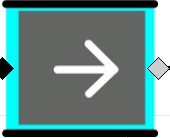
\includegraphics[scale=0.2]{inertia.png} & Inertia element is characterized by the $I$--intertance parameter and the relationship between pressure and solution flow of the two connectors:\\
 & $ q_{out}=-q_{in} $ \\
 & $ \frac{{\rm d}q_{in}}{{\rm d}t} = \frac{p_{in}-p_{out}}{I} $ \\
\hline
 \end{tabular}
 \caption{Icon and description of hydraulic components of Physiolibrary (21.). These are used, e.g., in order to model cardiovascular system.}
 \label{table:physiolibrary}
\end{table}

Once the model is formalized and constructed, a further problem is to estimate the model parameters so that the model reproduces a real world system. Without any further knowledge about the model, the problem of parameter estimation (or system identification) was shown to belong to the \emph{NP-complete} problems \cite{Hofmann2005}, which implies that the best known exact algorithm solving this problem has exponential time complexity. The heuristic methods (evolution strategies), randomization methods (Monte-Carlo method) and others are commonly used in order to find at least some parameter estimation in a reasonable time. Therefore, in further  work of this thesis an evolution strategy, genetic algorithm, was choosen as most robust for common models and system was proposed and implemented, which integrates this algorithm implemented in MATLAB environment and model simulation implemented in Modelica language.

The specific model of a studied system that is implemented in Modelica can be simulated in some Modelica tool. Or can be exported into a standard Functional Mockup Unit (FMU)\nomenclature{FMU}{Functional Mockup Unit}. Functional Mockup Interface (FMI)\nomenclature{FMI}{Functional Mockup Interface} defines FMU as a standardized XML\nomenclature{XML}{Extensible Markup Language} metadata description, packaged together with a binary library .DLL (or .SO), following a standardized API, published by Blochwitz et al. \cite{Blochwitza}\footnote{\url{https://www.fmi-standard.org/} accessed February 2015}. This API can be used to get/set values of model variables and to simulate the model.


%
%%The measurements are carried out in laboratories or in hospitals. Lumped parameter models are usually represented as ordinary differential equations and differential algebraic equations. They characterize the reality as a topology of discrete elements. The imaging methods for processing and analysis (section \ref{sec:imaging}) are used to construct 3D models from segmentation and generate mesh representations that are connected to physical principles. 


%
%%The application of mathematical modeling techniques towards biomedical research is sometimes called systems biology. This approach combines the reductionism and integration, as denoted by Kohl et al.\cite{Kohl2010}. Application towards clinical practice includes the quantification of the diagnostic index or treatment strategy. It is a goal to develop tools, database models and methods of several Physiome projects, e.g., VPH-Physiome project presented by Hunter et al.\cite{Hunter2009}.
%
%One of the earliest complex and integrative modeling efforts was a model of circulation and its regulation, which was published by Guyton et al. in 1972 \cite{Guyton1972}. It continues as a "Human Model" or "HumMod" via derivative and technological upgrades, as introduced by Hester et al. \cite{Hester2011systems,hester2011}, with a focus on integration efforts. A different approach of modeling the human physiology is to construct a database of smaller models, which focus on some particular physiological phenomenon. For example, the NSR Physiome project introduces a  JSIM\footnote{JSIM: \url{http://www.physiome.org/jsim/} accessed January 2015} Java-based simulation system in order to support modeling in  physiology. A repository of several hundred models was published using this system \cite{Butterworth2014}. A similar effort is made by the IUPS Physiome project and repositories of the models are  based on XML standard languages CellML and FieldML \cite{Hunter2004,Yu2011}. The Systems Biology Markup Language (SBML) is used for modeling a biological system at the level of biochemical reaction and regulatory network. Another database collects several hundreds of curated and non-curated models \cite{Hucka2004,LeNovere2006}. These in-house domain-specific language and tools (although standardized by several organizations) like JSIM, CellML and FieldML, SBML or HumMod, have reached their capabilities for representing complex models. Only the HumMod achieved the integrative approach, building a complex integrative model of human physiology using a lumped parameter approach. However, as the HumMod modeling technology is maintained by a small team of experts, it is not used in broader physiology community. Other authors use commercial or industry standard tools for mathematical modeling and computing. For example, Kofranek et al. described Guyton's 1972 model in MATLAB\textsuperscript{\textregistered} Simulink \cite{Kofranek2010} and the derivative HumMod in acausal object-oriented Modelica language \cite{Kofranek2011hummod,kofranek2013hummod}.
%
%

%
%
%\subsection{Modeling Methodology}
%\label{sec:methodsmodels}
%
%
%%The methodology of formalizing mathematical models is influenced by the abilities of underlying modeling language that is used. 
%%JSIM, CellML, SBML or HumMod are domain specific languages and the tools that are primarily developed within physiological or systems biological communities. 
%%Other authors use commercial or industry standard tools for mathematical modeling and computing. For example, Kofranek et al. described Guyton's 1972 model in MATLAB\textsuperscript{\textregistered} Simulink \cite{Kofranek2010} and the derivative HumMod in acausal object-oriented Modelica language \cite{Kofranek2011hummod,kofranek2013hummod}. Fernandez et al. described models of cardiovascular pulsatile system using MATLAB Simscape  \cite{FernandezDeCanete2013} and recently, in Modelica  \cite{FernandezdeCanete2014}.
%
%The Modelica language is an object-oriented, equation-based and acausal modeling language standardized and maintaned by the Modelica association\footnote{\url{http://www.modelica.org} accessed February 2015}.
%
%%finished writing of autoreferat 7th April.
%Therefore, I contributed to the modeling methodology beneficial for complex models, which key features are the acausal modeling technique and object orientation. This keeps the complex model structure decomposed into understandable and maintainable parts and allows the complexity of models like HumMod to be covered. 
%
%The paper \cite{Kulhanek2014Modeling} \emph{Modeling of Short-term Mechanism of Arterial Pressure in the Cardiovascular System: Object-oriented and Acausal Approach} in Appendix~\ref{app:modeling} published disputation about causal and acausal approach in using Modelica for modeling pulsatile cardiovascular system (CVS)\nomenclature{CVS}{Cardiovascular System} and possible enhancement for more complex models. 
%
%The paper \cite{Kulhanek2014mefanet} \emph{Simple Models of the Cardiovascular System for Educational and Research Purposes} in Appendix~\ref{app:simplemodelsd}, published detailed methodology of modeling lumped parameter pulsatile CVS in Modelica. 
%
%A common guide to the Modelica language and its capabilities can be found an the published works of Fritzson \cite{fritzson2002} and in the on-line works of Tiller \cite{Tiller2014}.
%
%
%\subsection{Identification of physiological systems}
%\label{sec:estimation}
%


% This procedure is sometimes called system identification and the objective of the parameter estimation is usually to minimize the following function (to find the least amount of differences between the predicted and measured values):
%\begin{equation} \label{eq:parameter} 
%f( \vec{p} ) = \sum_{i=1}^{n} ( M(t_{i},\vec{p} ) - d(t_{i}) )^2 \to min  
%\end{equation} 
%where $\vec{p}$ is the vector of values of parameters, $M(t_{i},\vec{p})$ is model simulated at time $t_{i} $ with the given parameter values $\vec{p}$ and $d(t_{i})$ is the measured experimental value at time $t_{i}$. 



%global optimization methods must be used in general, and ,
%, e.g. based on brute-force search -- trying all possible values of the parameters and simulate the model with them, finding the minimum of the objective function (\ref{eq:parameter}).
%Further reading about parameter estimation and system identification can be found in published works edited by Eykhoff \cite{Eykhoff1981}, or in the published works of Khoo \cite[p.~159]{khoo2000}.
%


%Evolution strategies have been identified as robust, having the potential to utilize parallel computing methods \cite{Moles2003}.
%
%Parameter estimation and further analysis methods are part of specialized mathematical software. For example, Pruet et al. used Metropolis algorithm to produce a distribution of parameters in order to calibrate a model of the human cardiovascular physiology. This was further tested against the predictive ability of circulatory failure and statistical methods were used with the software Wolfram \textit{Mathematica} \cite{Pruett2013}. The iterative improvement method in the MATLAB Simulink\textregistered ~was used by Takahashi et al. in their estimation of two parameters of a simple cardiovascular model \cite{Takahashi2013}. Furthermore, Abbas et al compared several methods in their estimation of multiple parameters of a cardiovascular system in MATLAB Simulink\textregistered \cite{Abbass2012}.
%
%Maffioletti et al. published a GC3Pie framework, which utilized evolutionary algorithms. They introduced workflow to identify parameters of models for economical predictions, using grid computing infrastructure \cite{maffioletti2012computational}. Humphrey et al. calibrated hydrology models, utilizing a commercial Windows Azure cloud computing infrastructure and achieved significant speedup \cite{Humphrey2012}.
%
%\subsection{Methods for Parameter Estimation}
%\label{sec:methodsestimation}
%
%\begin{figure}[htb]
%    \centering
%    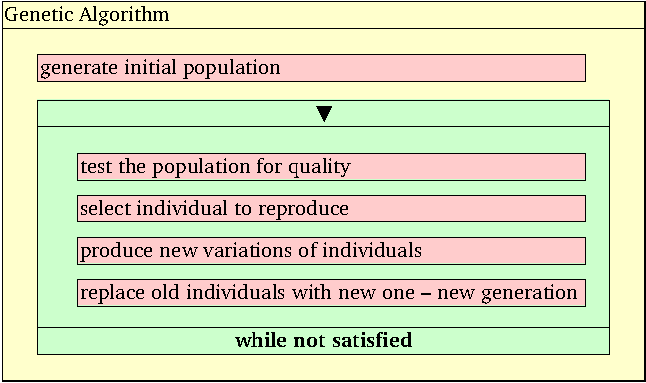
\includegraphics[page=1]{chapter3/GA-kopenogram-crop.pdf}    
%%    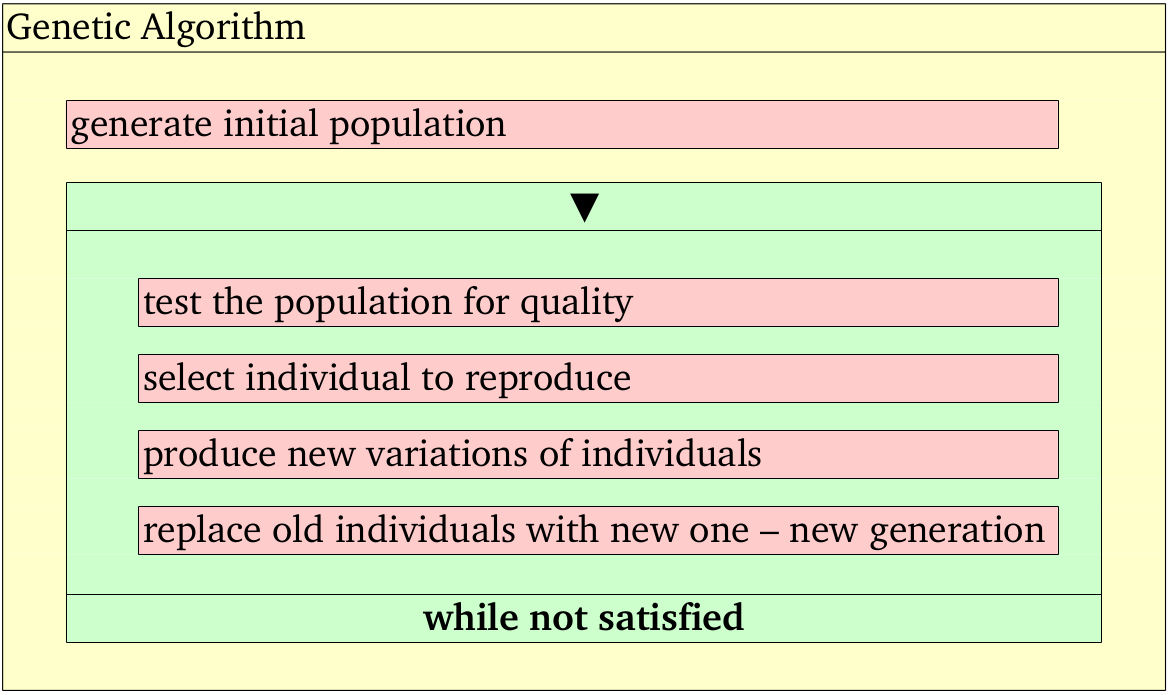
\includegraphics[width=0.5\textwidth]{chapter6/GA-kopenogram.png}
%    \caption{Kopenogram of a genetic algorithm. 
%    }
%    \label{fig:GA-kopenogram}
%\end{figure}
%
%An evolutionary algorithm can be used as a heuristic strategy for finding global minimum or maximum. It can also be used to estimate the parameters of a model. A genetic algorithm is a type of evolutionary algorithm, which encodes individuals as binary string. It was introduced by the likes of Holland\cite{Holland1975}. These algorithm steps are schematically presented in Figure \ref{fig:GA-kopenogram}.
%
%\begin{figure}[htb]
%    \centering
%    \includegraphics[page=2]{chapter3/GA-kopenogram-crop.pdf}    
%%    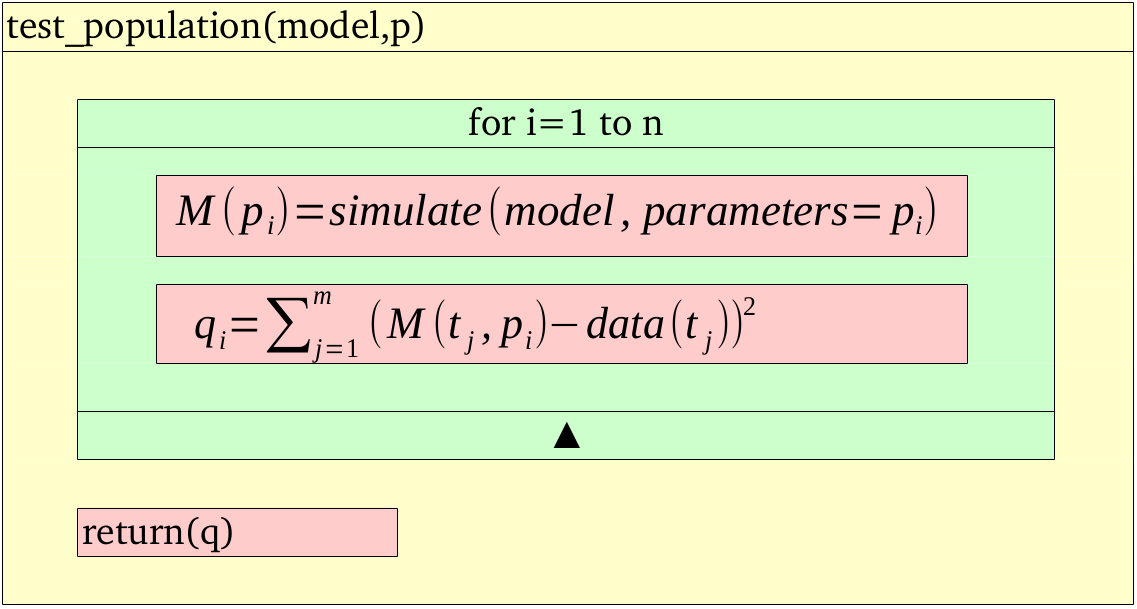
\includegraphics[width=0.5\textwidth]{chapter6/GA-kopenogram2.png}
%    \caption{Kopenogram of the specific test of a population for quality, in the case of parameter estimation used by a genetic algorithm. The model is simulated according to individual $i$ with parameters $p_i$ and the quality $q_i$ is counted per the objective function \ref{eq:parameter}.
%    }
%    \label{fig:GA-kopenogram2}
%\end{figure}
%
%The iteration within the loop "$\blacktriangledown \ldots$ \emph{while not satisfied}" depends on the previous iteration and, thus, it cannot be parallelized. However the \emph{test the population for quality} has an algorithmical structure in Figure \ref{fig:GA-kopenogram2} for the parameter estimation. Each iteration in the loop "\emph{for i=1 to n}" is independent and, therefore, loop parallelism (section \ref{sec:parallelprogramming}) can be utilized and implemented here.
%
%\subsubsection{Architecture of System for Parameter Estimation}

%
%The parallelization is implemented using threads. For this, in \emph{test\_population} method is used, which, within a loop, follows a fork/join pattern -- the created threads simultaneously ask for simulation results with a parameter set and the main process waits until all of the results are returned before computing the full vector of quality evaluation $q$.
%
%Model specific FMU is packaged with a .NET ServiceStack framework\footnote{\url{https://servicestack.net/} accessed February 2015} and it exposes a simulation functionality as a RESTful web service, which can be accessed and orchestrated by the \emph{test\_population} algorithm. The implementation of genetic algorithm is reused from MATLAB \texttrademark Global Optimization Toolbox\footnote{\url{http://www.mathworks.com/products/global-optimization/} Matlab Global Optimization Toolbox, accessed March 2015} and, with a database of results in a SQL database, is integrated with an ASP.NET web application. This presents a web user interface and functionality to a user. Section \ref{sec:resultsestimation} describes the results of applying the methods and deploying the designed system in a local cluster and cloud computing infrastructure.
%
%\subsection{Parameter Sweep}
%\label{sec:sensitivity}
%After the parameter estimation, further problem arise regarding the structural identifiability and analysis of sensitivity to the estimated parameter values\cite[p.~176]{khoo2000}. 
%
%\begin{figure}[hbt]
%    \centering
%     \includegraphics[page=4]{chapter3/GA-kopenogram-crop.pdf}    
%%    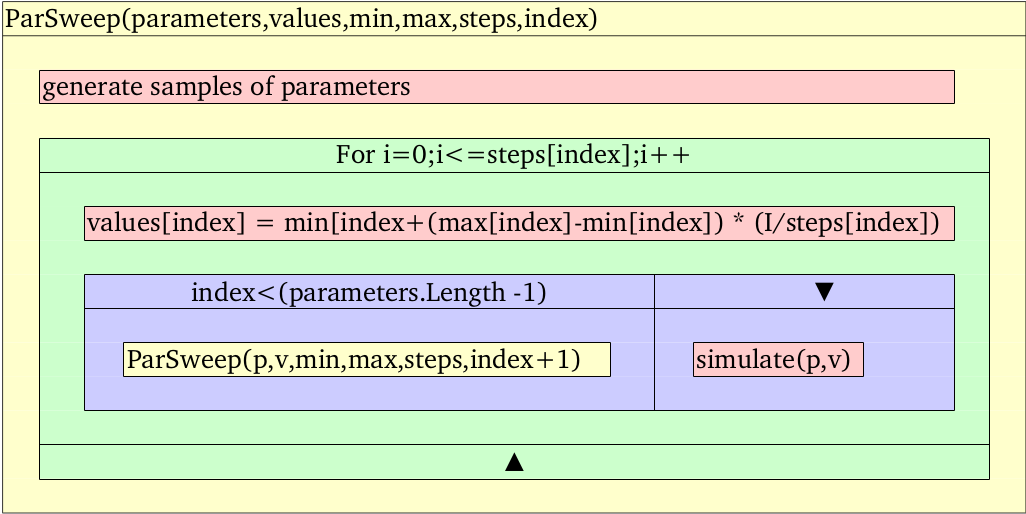
\includegraphics[width=1\textwidth]{chapter3/paramsweepkop.png}
%    \caption{Kopenogram of a recursive parameter sweep algorithm. $p$,$v$,$min$,$max$ and $steps$ are arrays with the same dimension that hold the parameter name, value, starting and stopping value and number of steps that have to be performed between the starting and stopping value per each $index$.    
%    }
%    \label{fig:paramsweep}
%\end{figure}
%
%Parameter sweep (PS) is one of the techniques that is used for a sensitivity and uncertainty analysis, which is based on the changing selected parameters, simulating whole model and quantifying the change on model behavior with different parameters. An uncertainty and sensitivity analysis tries to determine how a change in the value of a parameter  contributes to the model output and how the estimation of parameter values is robust against errors of real data measurement. The various methods for carying out an uncertainty and sensitivity analysis have been published, e.g., in reviews by Helton et al. \cite{Helton2006} or in publications by Saltelli et al.\cite{Saltelli2004,Saltelli2008}. 
%
%The recursive algorithm of a parameter sweep for exploring parameter space (in Figure \ref{fig:paramsweep}) generates a tremendous number of simulations. Presuming that \emph{simulate} operation takes a constant time for any parameters (which, in general, is not true), the time complexity of PS is exponential $O(\prod_{i=1}^{n}) \text{steps}_i) \approx  O(k^n)$ where $k=\max_{i=1}^n(\text{steps}_i)$ and $n$ is number of parameters to be swept. For example, for 1~000 values for each parameter: $O(1000^n)$. The large number of distinct simulation can take a tremendous ammount of time on a single computer. However, in contrast to parameter estimation, each simulation is independent and a PS algorithm is determined as embarrassingly parallel. It is implemented in many grid computing projects and workflows, e.g., P-Grade portal, as published by Kacsuk et al.\cite{Kacsuk2011}.
%
%A system was proposed with customized BOINC platform\cite{Anderson2004}\footnote{\url{http://boinc.berkeley.edu/} accessed February 2015}. The task parallelism and master/worker programming model (mentioned in section \ref{sec:parallelprogramming}) is utilized. The Modelica model exported as FMU for Windows platform is integrated with BOINC wrapper. As a whole, it is integrated into BOINC platform, which is deployed on a server, as seen in Figure \ref{fig:paramsweeparch}. 
%
%\begin{figure}[htb]
%    \centering
%     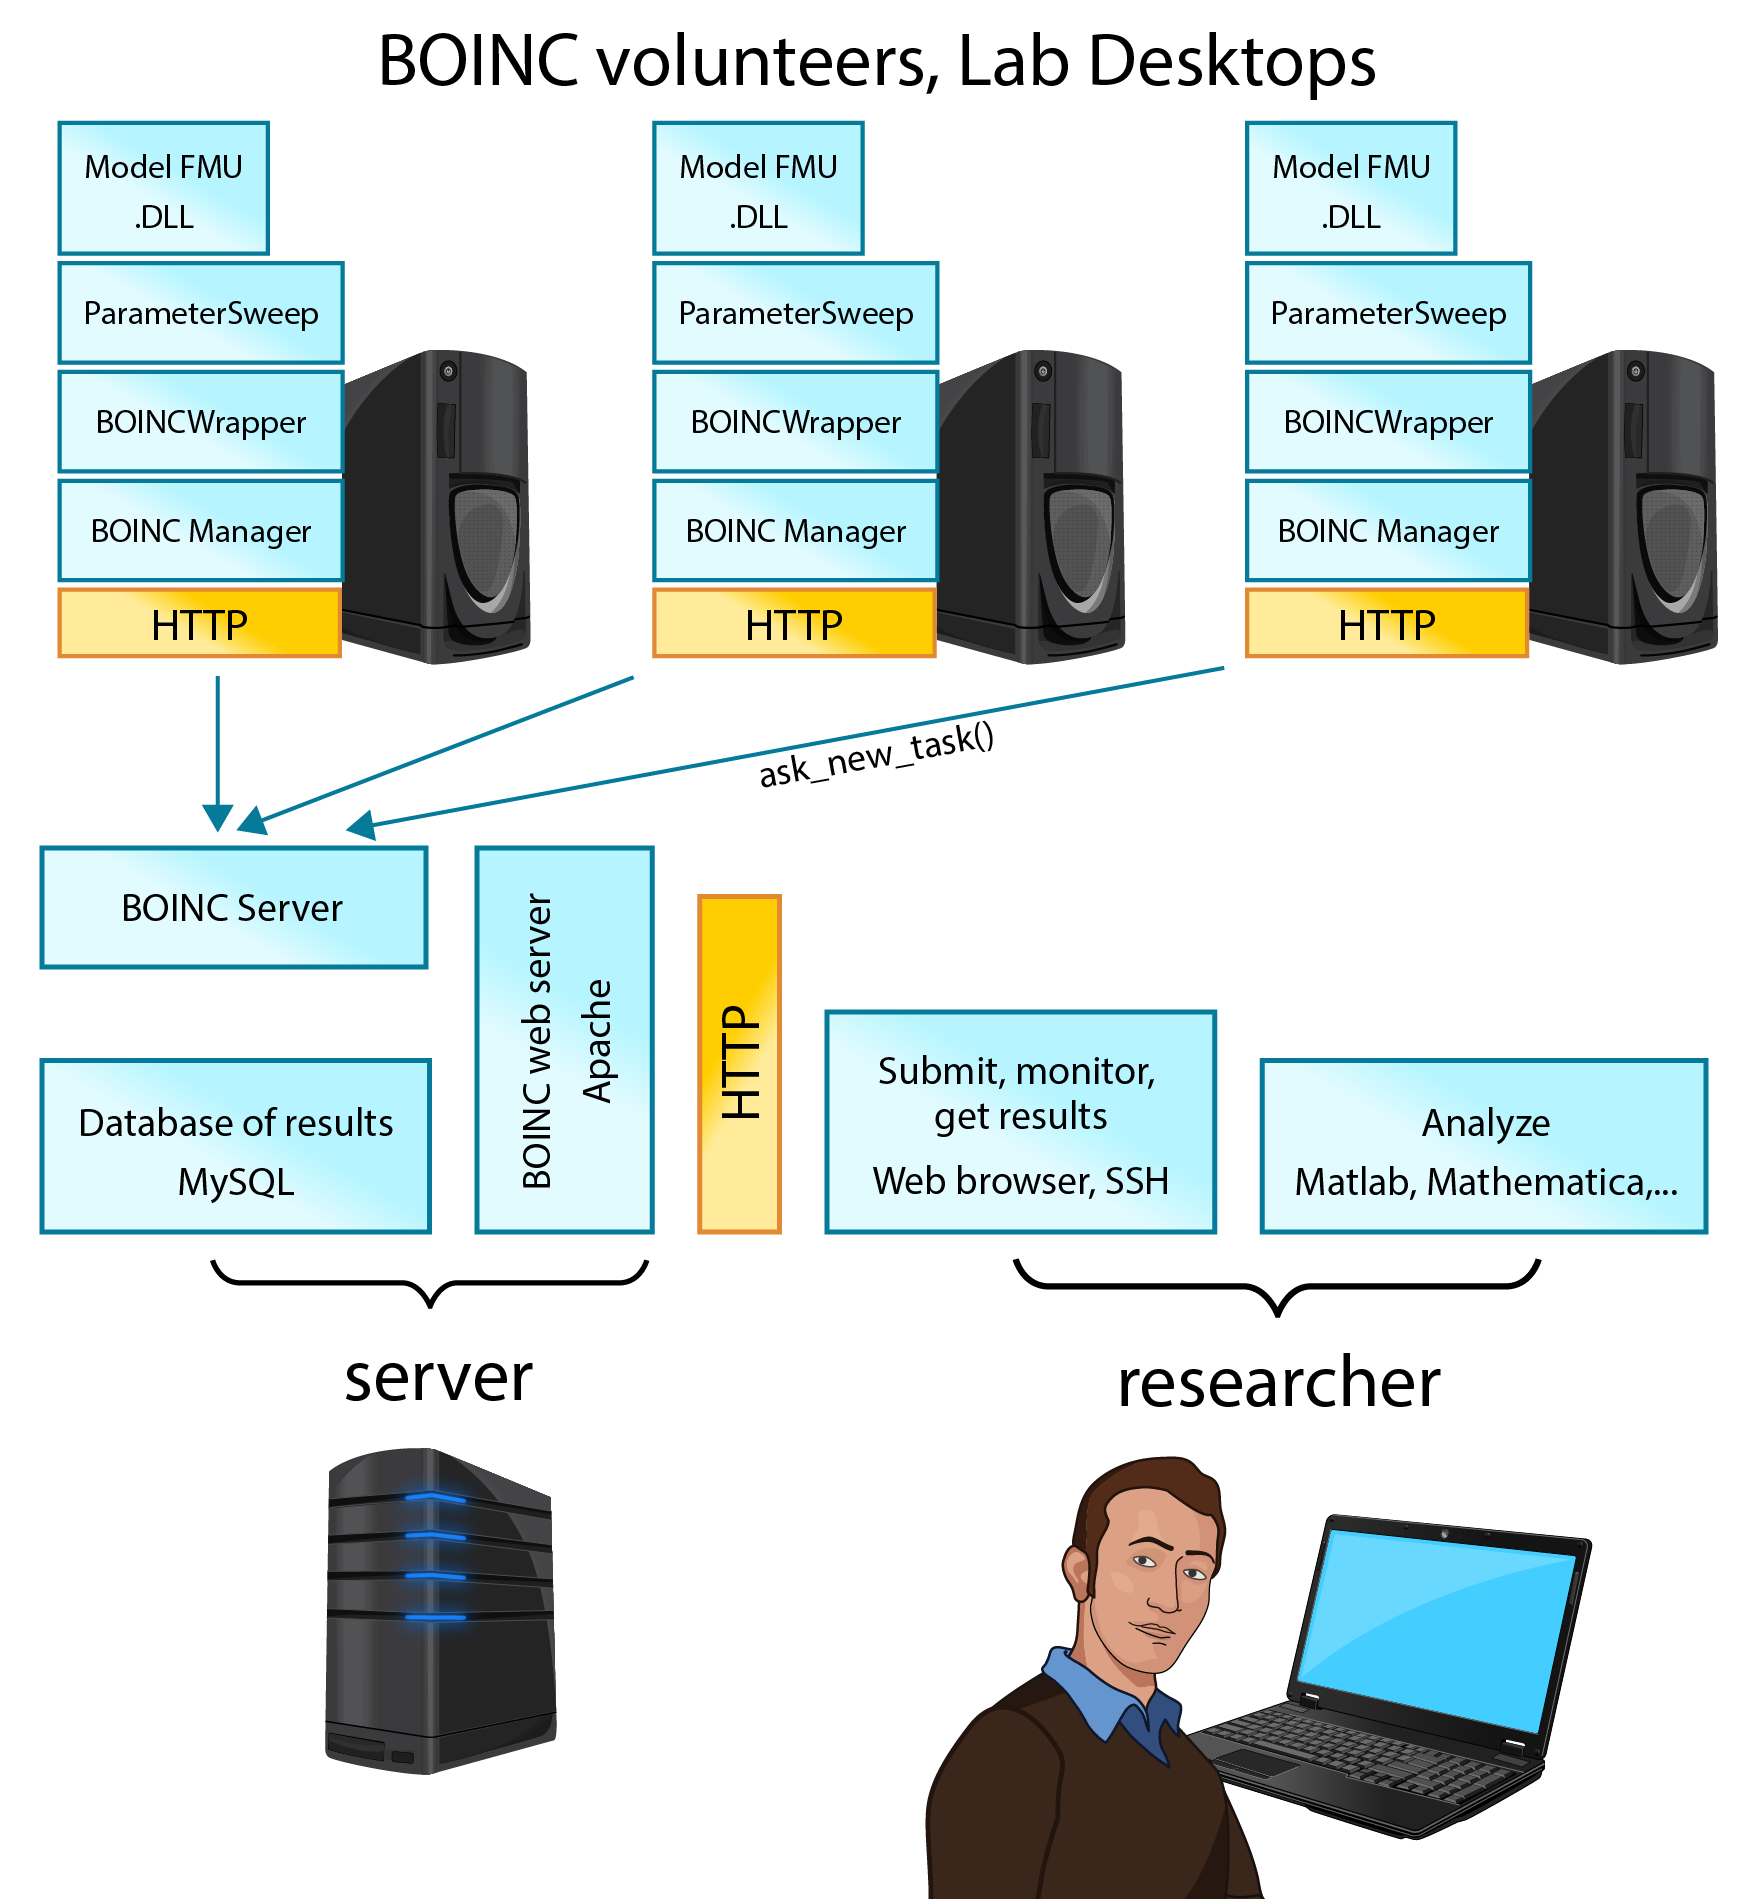
\includegraphics[width=0.75\textwidth]{img/chapter3-architekturaparamsweep-01.png}    
%%    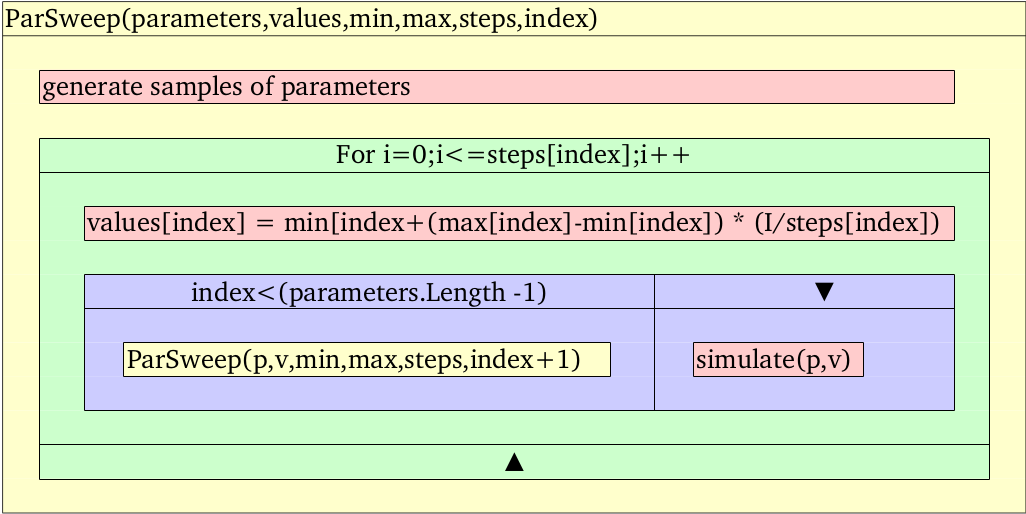
\includegraphics[width=1\textwidth]{chapter3/paramsweepkop.png}
%    \caption{Architecture of a parameter sweep integrated into BOINC framework. The whole parameter space is divided into smaller spaces which are resolved by the BOINC workers}
%    \label{fig:paramsweeparch}
%\end{figure}
%
%The results are described in section \ref{sec:resultsestimation}.
 %methods
\chapter{Results}
\label{sec:results}
%In previous chapters, there were introduced different methods available for selected use cases in research in biology and medicine. 
%\section{Virtual Infrastructure}
%\label{sec:resultsinfrastructure}
The pilot virtual infrastructure dedicated for research purposes, as proposed by the author of this thesis (3.), was established to consolidate and share resources among different projects. 
%The paper \cite{kulhanek2010c} \emph{Infrastructure for Data Storage and Computation in Biomedical Research} in Appendix~\ref{app:infrastructure} describes result of establishing the virtualization on physical infrastructure to share computational power among different platforms.
\section{Medical Image Sharing}
\label{sec:resultsimages}

The pilot infrastructure of several servers was installed in several institutions in Prague, Czech Republic. Globus Toolkit and Globus MEDICUS were installed on them,
the system connected with MEDIMED project integrates classical production system to share medical images with grid-based PACS system via the DICOM protocol. The grid-based system was tested with about 1300 DICOM records and enhanced with simple DICOMViewer available as web application. 
The grid-based solution allows to store large set of data records and manage replicas. The standard protocol to transfer data files gridFTP allows to effectively transfer parts of the files to the desired location from existing replicas within grid infrastructure to a desired location where an image processing can be performed. Current systems of sharing medical images may suffer from the problem of single point of failure or bottleneck. The grid-based solution brings robustness against the mentioned problems. 

\section{Remote Voice Analysis}
\label{sec:resultsvoice}

RDP protocol was customized and support for transferring sound recording was implemented. A client plugins were customized for the Linux "rdesktop" application as well as for the Windows default "tsclient" application. The plugin initiates sound recording from a sound device and creates a custom RDP channel. A raw data obtained from the sound device is transferred to the custom RDP channel. The server plugin writes the data from the custom channel directly to a file in WAV format and offers sound samples to the analytical application for real-time processing. The schematic architecture of the system is in Figure \ref{fig:architecturesound}.

\begin{figure}[hbt]
    \centering
     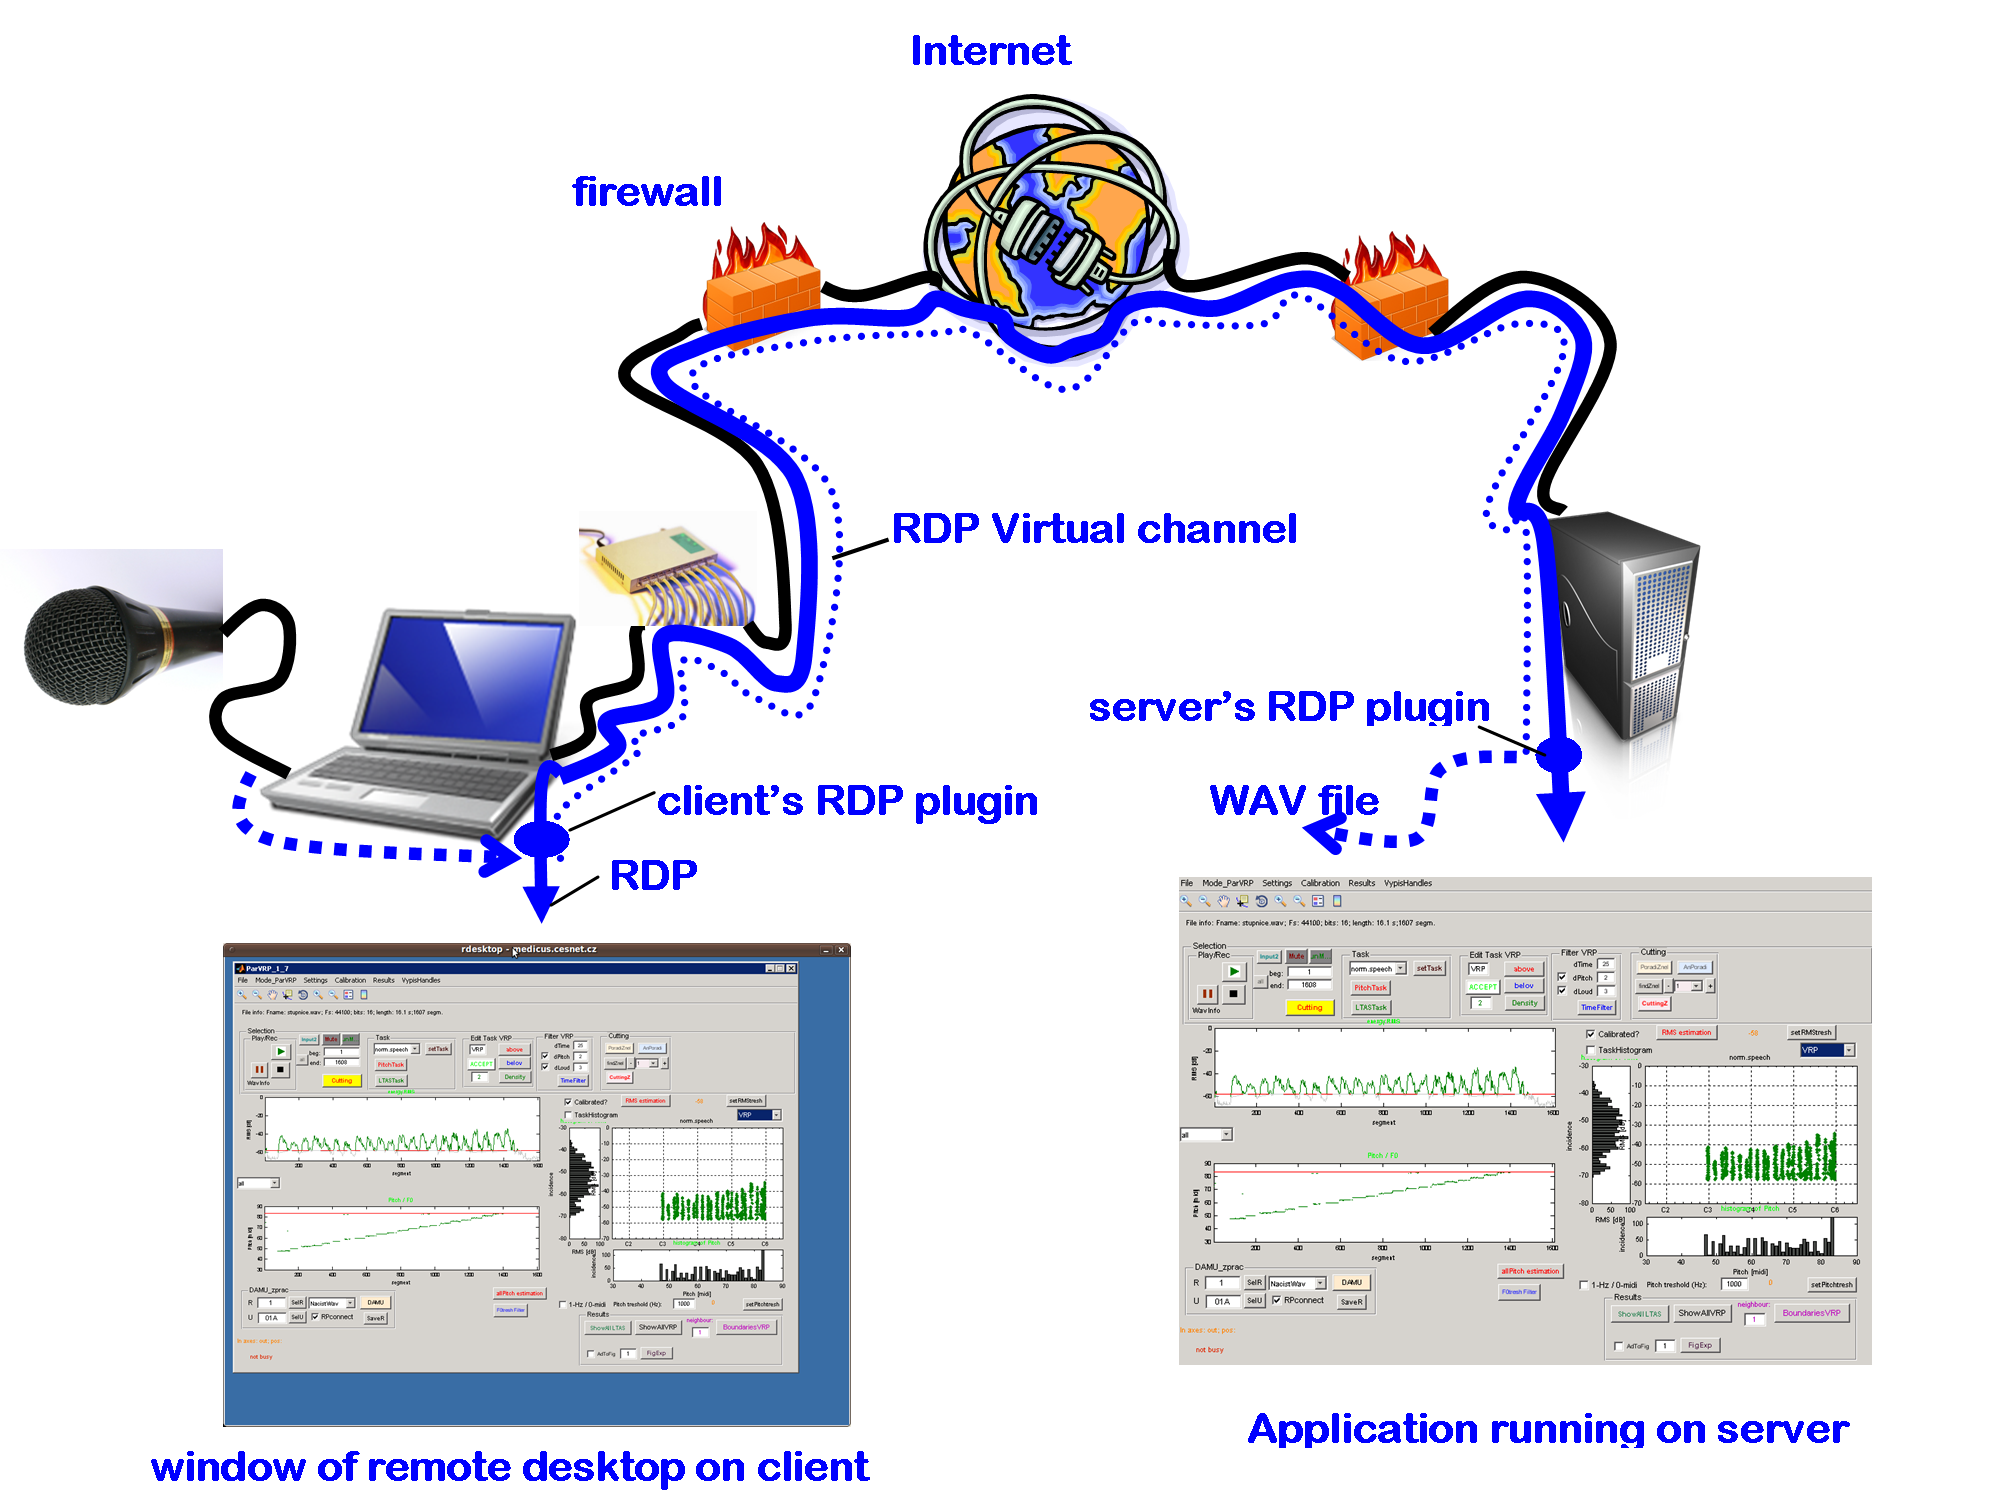
\includegraphics[width=0.75\textwidth]{schemasystemu.png}  
    \caption{Architecture of a system for remote voice analysis and RDP plugins for sound recording redirection.}
    \label{fig:architecturesound}
\end{figure}

The default sound recording features of RDP protocol version 5.2 and 7.0 degrades sound quality transferred to the server application, furthermore, some samples of the sound were lost and sound become garbled or scratchy. The sound quality using the custom RDP channel is without loss of information and acceptable for further analysis. Additionally, the remote application with custom RDP plugin was packaged as a virtual machine template and can be provisioned on cloud computing infrastructure in case of the need.

The application allows to record the voice of patient, the voice signal is transferred to remote application where it is processed and analyzed, the results are visualized in real-time. The application is now used by several voice therapists and voice pedagogues in different areas of the Czech Republic and Slovakia to analyze the voice in non-invasive way in order to see e.g. the progress of the voice training methods.

\section{Computational Physiology}
\label{sec:resultsestimation}

\subsection{Modeling Methodology}

Within the thesis, the modeling methodology was improved in an area of modeling cardiovascular system in a complex integrative way, which can be used for research and educational purposes. A set of recommendation was published: (1) to use acausal connector (special purpose class where no causality (what is input and output) is defined), (2) utilize object-oriented features in order to separate pure model from the specific experiment, (3) combine textual and diagram notation in order to express mathematical equations/component relations.
%The modeling tool will decide the direction of computation (what will be input and output) upon compilation time. 
This lead to more exact and understandable model for domain experts. 
The table \ref{table:physiolibrary} contains definition of basic components of hydraulic domain used to model cardiovascular system. Figure \ref{fig:fernandezmodel} shows an  implementation of the model published originally by Fernandez de Canete \cite{FernandezDeCanete2013} in Modelica language published in (7.). Such medium complex models are important for further studies. Methodology and it's usage in education is described in publication by the author of this thesis in (1.) and (7.).


\begin{figure}[ht]
    \centering
    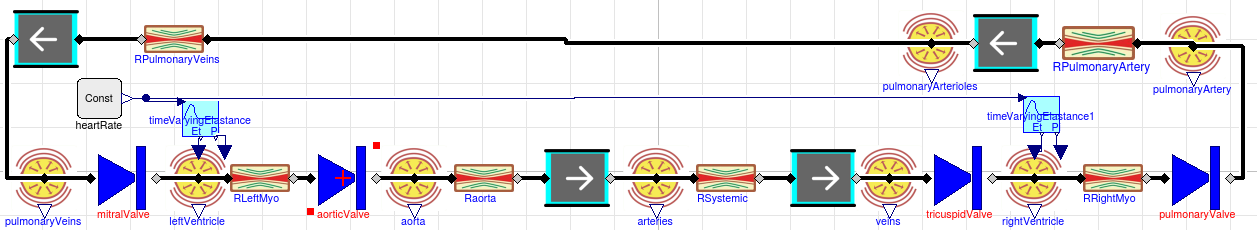
\includegraphics[width=1\textwidth]{fernandezmodel.png}
    \caption{Implementation of the model of cardiovascular system \cite{FernandezDeCanete2013} in Modelica language using components of Physiolibrary (21.). The connected components is compiled by the Modelica tool with the equation defined in Table \ref{table:physiolibrary}. In this case the 209 equations (133 are trivial and 76 are non-trivial equations) are generated and causality is solved by the tool.
    }
    \label{fig:fernandezmodel}
\end{figure}

%A set recommendation regarding causal and acausal approach in using Modelica for modeling pulsatile cardiovascular system (CVS)\nomenclature{CVS}{Cardiovascular System} was published in (1.) and implementation of cardiovascular system controlled by the baroreceptor control system was implemented showing robust solution.

\subsection{Parameter Estimation}

The proposed architecture of the system for parameter estimation (Figure  \ref{fig:architectureestimation}) was influenced by the need of some interactivity and for the overall accessibility for users, which is fulfilled by the web UI. 

\begin{figure}[hbt]
    \centering
     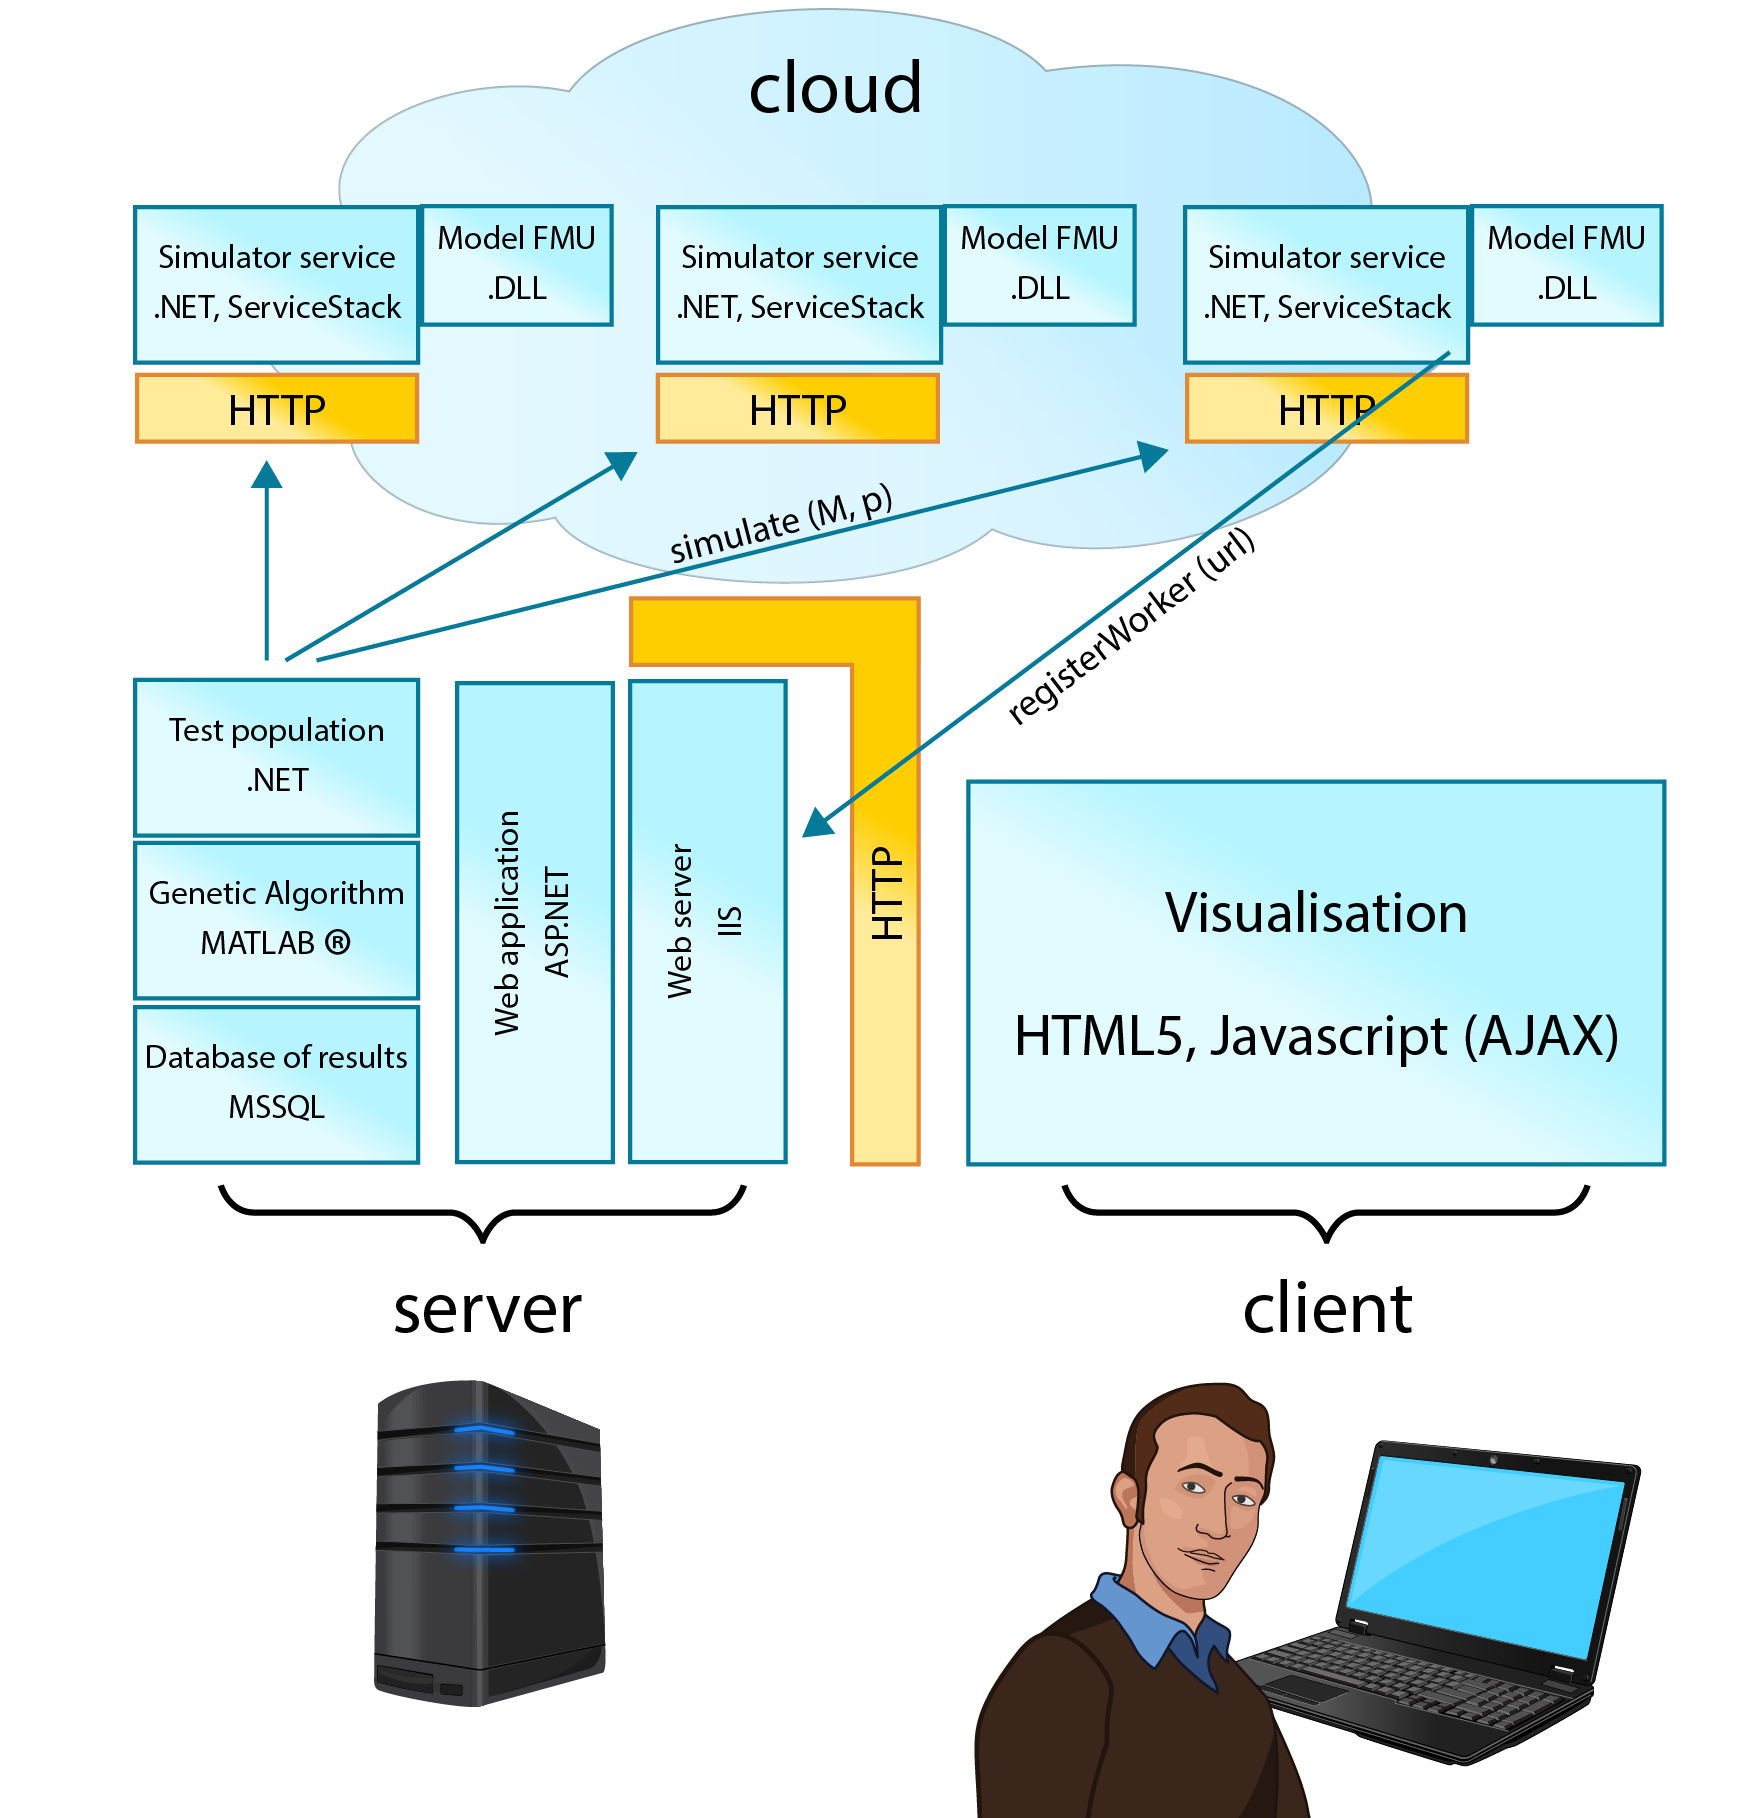
\includegraphics[width=0.75\textwidth]{../img/chapter3-architekturaestimation-01.png}  
    \caption{Architecture of a system that employs genetic algorithm and distributes the task \emph{simulate} into a cloud computing environment.}
    \label{fig:architectureestimation}
\end{figure}

The Modelica models is exported to standardized FMU and wrapped with a RESTful webservice implemented in .NET ServiceStack framework\footnote{\url{https://servicestack.net} accessed April 2015} allowing remote control of simulation. In the time of writing this thesis, the most stable Modelica tool was Dymola version 2015\footnote{\url{http://www.dynasim.se} - Dymola tool, accessed March 2015}, and most stable export was to FMU for a MS Windows platform. Several RESTful web services packaged in a virtual machine template was instantiated in scientific cloud.
The overall performance and speedup estimation were tested against the Modelica implementation of complex physiological model HumMod \cite{Kofranek2011hummod}, the Modelica implementation of a model of hemodynamics of the cardiovascular system, originally published by Meurs \cite{Meurs2011} and the model of $O_2$, $CO_2$ and $H^+$ binding on hemoglobin, published by Matejak et al. and contributed by the author of this thesis (2.)%\cite{Matejak2014sj} 

\sisetup{round-mode=figures,round-precision = 3}
\begin{table}[htb]
\footnotesize
\begin{tabular}{|l|r|r|r|r|r|r|r|r|r|}
\hline
compl. & name & S(10) & S(20) & S(30) & S(40) & S(50) & S(60) & S(80)& S(160)\\
\hline
high & HumMod \cite{Kofranek2011hummod} & $\num{10}$ & $\num{20.4}$ & $\num{24.8}$ & $\num{35.4}$ & $\num{41.8}$ & $\num{49.83}$ & $\num{63.9807249802}$ & $\num{121.5389821285}$ \\
medium & Meurs2011\cite{Meurs2011} & $\num{8.7}$ & $\num{16.6}$ & $\num{24.4}$ & $\num{29.6}$ & $\num{32.9}$ & $\num{38.65}$ & $\num{55.9311360464}$ & $\num{53.0128125}$ \\
low & Matejak2014\cite{Matejak2014sj} & $\num{7.5}$ & $\num{11.8}$ & $\num{12.5}$ & $\num{15.4}$ & $\num{15.7}$ & $\num{14.73}$ & $\num{16.6865881526}$ & $\num{12.5500720509}$\\ \hline
\end{tabular}
\caption{Comparison of model scalability and complexity. Speedup $S$ on 10 CPUs till 160 CPUs of parameter estimation, using cloud computing cluster on 1-6 virtual machines, each 10 CPUs (2x5-core Intel E5-2620 2GHz, 1Gbit/s Ethernet.) (resp. 5-10 virtual machines, each 16 CPUs on physical hardware 2x 8-core Intel E5-2670 2.6GHz). Genetic algorithm configured with a population $120$ (resp. $640$) individuals for $10$ (resp. $20$) generations. Speedup estimated from measuring the serial computation on 1 CPU.}
\label{table:speedupresult3}
\end{table}

To summarize the results from Table \ref{table:speedupresult3}, the low complex model scales up to 40 CPUs with a speedup of 15. The medium complex model scales up to 80 CPUs with a speedup of 56 and complex model scales up to 160 CPUs (and probably more) with a speedup of 122. Practically, good parameter estimation was obtained after 200 generations with population of 640, which implicates that the computation time can be reduced from four days to 47 minutes in the case of complex model and from 14 hours to 15 minutes in the case of medium complex model.

The parameter estimation on low complex model suffers with major network overhead. Thus, such low complex models can be effectively identified on local cluster with comparable time of computation.

\section{Adair-based Oxygen Binding to Hemoglobin}
The parameter estimation was used to compute parameters of newly constructed model of hemoglobin integrating $O_2$ , $CO_2$ and $H^+$ binding based on theoretical principles, which were verified on the parameter estimation algorithm system described above and noted as the low complex model Matejak2014 published as (2.).
The author of this thesis implemented the model in Modelica language and estimated parameters of dissociation constants of the chemical reaction of oxygen binding to different forms of hemoglobin comparing the simulated saturation curves of $O_2$ with the experiments published in scientific literature.

\section{Parameter Sweep}
The desktop grid BOINC framework was customized and a system was established for parameter sweep application. The established project, \emph{Physiome@home}, and it's project web page, \url{http://physiome.lf1.cuni.cz/ident3/physiome}, manages workunit tasks which are downloaded and executed by BOINC workers. The worker application consist of a packaged model that is exported as FMU for a Windows platform and of a universal preconfigured wrapper application provided by BOINC framework, which integrates generic application with a BOINC manager on the desired volunteer computer. Workunits are generated by a tool within BOINC framework.

Parameter sweep method can enhance the ability to perform identifiability and uncertainity analysis of general complex models and can deliver results of explored parameter space in a reasonable time.

%\section{Parameter Sweep}
%\label{sec:resultsboinc}

 %results
\chapter{Discussion}
\label{sec:discussion}

%The result presented in section \ref{sec:resultsimages} is an example how a standard format and protocol DICOM is utilized to integrate current production system in order to exchange medical images (MEDIMED \cite{Slavicek2010}) and a grid-based solution (Globus MEDICUS \cite{Erberich2007}). Remote Desktop Protocol (RDP) is a key standard for protocol in order to integrate the application of voice analysis\cite{Fric2007} into a remote environment, which is accessible via the Internet. This is presented in section \ref{sec:resultsvoice}. In the case of parameter estimation, a key factor is the standard Functional Mockup Interface (FMU)\cite{Blochwitza},  which allows the control and simulation of a physiological model in a customized tool that is not related to modeling tool. This is presented in section \ref{sec:resultsestimation}. 

%The selection of a joint element increases the chances of reusability of such a system in future development, when requirements usually change and the reconstruction of a system or architecture is needed. For example, 

The presented solution, which is based on Globus MEDICUS, is, in general, a data warehouse, that stores one or more copies of DICOM images. However, federated files and metadata that are stored within home institutions, which only share network infrastructure to interchange the DICOM studies, seems to be a preferred and more acceptable solution by hospitals today, as published by Chervenak et al. \cite{Chervenak2012}. The grid computing infrastructure seems to be suitable for research and educational purposes, but not generally acceptable for clinical use. 
 
In the case of remote voice analysis, the remote access to an application keeps the majority of user experience via network protocol, as presented in section \ref{sec:resultsvoice}. It is a way how to migrate legacy application into the computing infrastructure and how to offer it as a service via network protocols. Cloud computing allows to instantiate the virtual machine with such service on demand.

% Such service can be deployed on any web server and the occasional need to educate or perform a higher number of analysis concurrently can be satisfied with cloud computing deployment. 
%The application process for sound signal which is currently analyzed by Fast Fourier Transformation algorithm quite effectively. Another challenge is to analyze a sound signal connected with high-speed video or videokymography methods, which need to transfer, process and store larger amounts of data. 

In the case of the application for parameter estimation presented in section \ref{sec:resultsestimation}, the computation is sensitive on communication overhead. For simple models, local high performance computing (HPC) resources are most beneficial. For medium and highly complex models, the deployment of worker nodes into a cloud computing environment is worth considering. Another challenge is to estimate optimal size of population for genetic algorithm in order to optimize computational time and reduce suboptimal results, as proposed by Gotshall et al.  \cite{Gotshall2000}.

The parameter sweep problem is considered as embarrassingly parallel and highly suitable for high throughput computing (HTC), which is the main focus of current grid computing infrastructures. 

When porting an application to a grid environment, one of the important decision is the platform of the used system, which is sometimes hard to involve, e.g., within the thesis the were available code from a third party tool for the MS Windows platform only. This can determine the platform of the worker node and the virtualization - or, in the case of parameter estimation, cloud computing is utilized on a prepared platform. In the case of parameter sweep, a desktop grid computing BOINC worker and application for a MS Windows platform is prepared for volunteers with the compatible system. To utilize the service grid infrastructure, an export of the model into a FMU library and implementation of the wrapper service must be done in the grid computing platform, which is usually a Linux based system. An option can be to use WINE\footnote{\url{https://www.winehq.org/} WINE. Accessed March 2015} -- a compatibility layer that is capable of running Windows applications on several POSIX-compliant operating systems, such as Linux, Mac OSX and BSD. This would allow utilizing traditional service grid infrastructure for, e.g., parameter sweep application having an advantage not to maintain the desktop grid BOINC server.

For smaller types of application and scientific community with their own tools, the question is, whether or not to invest on porting their tools to grid specific platform and parallel programming model. 
In the case of integrating with a service grid middleware or with desktop grid framework, expert knowledge is needed to configure and customize the system. This is the case for the sharing of medical images (section \ref{sec:resultsimages}) and for parameter estimation and parameter sweep, which was tried with the desktop grid approach - BOINC framework.% (section \ref{sec:resultsboinc}).

Virtualization facilitates the integration effort, as presented in the case of remote analysis of the human voice (section \ref{sec:resultsvoice}) and in the case of deployment of worker nodes in a cloud computing environment for parameter estimation (section \ref{sec:resultsestimation}). 

Based on previous results and ideas, the answer to the research questions can be formulated:
\begin{itemize} 
\item \emph{Is it beneficial to utilize grid computing and cloud computing technology for the processing of medical information and how?}

Grid computing and cloud computing can significantly speedup parameter study of medium and complex models in computational physiology. Such a speedup could influence its applicability in clinical use. %, it was shown that parameter study of the medium and complex models can highly benefit from grid-computing and cloud-computing environment. For the simple models only HPC resources with reduced communication overhead might be beneficial too. 
For the case of sharing and processing medical images or analysis of voice signals, grid computing or cloud computing introduces technology that facilitates cooperation among a community of users from different geographically dispersed areas and facilitates the sharing of large data sets.

\item \emph{What are the limitations of processing medical information in grid or cloud?}

Limitation are given by the effort needed to integrate or port an application carry out computation or share data. The cost of porting an application to cloud computing is reduced by virtualization technology, rather than to a grid computing environment, which needs additional work in order to adapt the application for a grid computing platform and API. 

The limitation are given by the theoretical features of algorithms too. Grid computing and cloud computing are not general solutions for hard problems (NP-complete problems). With connected with non-exact methods, a concurrent processing of many tasks may bring an acceptable non-exact solution.

\item \emph{How can the grid computing and cloud computing influence the direction of biomedical research?}

The fact that the computation or data are processed remotely is one of the paradigm shift. The data moves from files stored in some folder to elements or objects living somewhere on server or cloud which can be shared among researchers. 
 
% proposed a noninvasive method based on computational fluid dynamic and magnetic resonance imaging (MRI) to identify pressure difference in aorta for further hemodynamics analysis based on four element windkessel model. However, such type of studies usually focus on particular phenomenon and tries identify parameters of very simplified models that are currently known in systems biology domain. In the time of writing this thesis, 

%And the grid-based or  cloud-based medical data management solution can be used as technology and infrastructure to store and share the expected big ammount of raw scientific results, such as images or videos. 
%Several computational and storage demanding biomedical application were shown in animal models by Saritas et al.\cite{Saritas2013}. 
The research infrastructures, e.g. Integrated Structural Biology Infrastructure for Europe (INSTRUCT)\footnote{\url{https://www.structuralbiology.eu/} accessed March 2015}, European Life Science Infrastructure for Biological Information (ELIXIR)\footnote{\url{http://www.elixir-europe.org/} accessed March 2015},  European Biomedical Imaging Infrastructure (Euro-BioImaging)\footnote{\url{http://www.eurobioimaging.eu/} accessed March 2015} and others rely on grid-computing and cloud-computing infrastructures for science. The purpose of these initiatives is to understand high-level phenotypes from genomic, metabolomic, proteomic, imaging and other types of data. They also require multi-scale mathematical models and simulations, as noted e.g. by Hunter et al. \cite{Hunter2013} in his strategy for Virtual Physiological Human (VPH)\footnote{\url{http://www.vph-institute.org/} accessed March 2015}. 

The integration with multidimensional models of geometrical, mechanical properties and the time-dependence of the compartment's data, which is taken from medical and biological repositories, can highly improve complex models of human physiology which are based mainly on lumped-parameter approach. E.g. Itu et al. achieved parameter identification on simplified windkessel model of hemodynamics in order to study aortic coarctation, which is based on processing of MRI, and requires 6-8 minutes of computation time on a standard personal computer \cite{Itu2013}. One of the challenge of systems biology approach, as identified by Kohl et al. \cite{Kohl2010}, is to use multiparameter perturbation to identify the safe areas, e.g., for multitarget drug profile. The results presented in section \ref{sec:resultsestimation} shows that the parameter study can be done on much more complex models in a reasonable time. The computation is able to become practical for clinical and further research towards patient-specific health care, in silico trails and drug discovery. 
%The research infrastructures, e.g. Integrated Structural Biology Infrastructure for Europe (INSTRUCT)\footnote{\url{https://www.structuralbiology.eu/} accessed March 2015}, European Life Science Infrastructure for Biological Information (ELIXIR)\footnote{\url{http://www.elixir-europe.org/} accessed March 2015},  European Biomedical Imaging Infrastructure (Euro-BioImaging)\footnote{\url{http://www.eurobioimaging.eu/} accessed March 2015} and others, which technologically rely on grid-computing and cloud-computing infrastructures for science. The purpose of these initiatives is to understand high-level phenotypes from genomic, metabolomic, proteomic, imaging and other types of data. They also require multi-scale mathematical models and simulations, as noted e.g. by Hunter et al. \cite{Hunter2013} in his strategy for Virtual Physiological Human (VPH)\footnote{\url{http://www.vph-institute.org/} accessed March 2015}. 
%corrected April 3th
%The integration with multidimensional models of geometrical, mechanical properties and the time-dependence of the compartment's data, which is taken from medical and biological repositories, can highly improve complex models of human physiology which are based mainly on lumped-parameter approach. E.g. Itu et al. achieved parameter identification on simplified windkessel model of hemodynamics in order to study aortic coarctation, which is based on processing of MRI, and requires 6-8 minutes of computation time on a standard personal computer \cite{Itu2013}. On of the challenge of systems biology approach, as identified by Kohl et al. \cite{Kohl2010}, is to use multiparameter perturbation to identify the safe areas, e.g., for multitarget drug profile. The results presented in section \ref{sec:resultsestimation} shows that the parameter study can be done on much more complex models in a reasonable time. The computation is able to become practical for clinical and further research towards patient-specific health care, in silico trails and drug discovery. 

%Additionally, it is a business strategy of several new ventures in order to collect anonymized patient records from clinicians, to gradually improve diagnostic methods and to provide reciprocal services for supporting clinical or therapeutic decision, as presented in section \ref{sec:resultsvoice}. For example,  Fetview\footnote{\url{http://fetview.com/} accessed March 2015} is an startup company, which one aim is to support fetal healthcare and gradually improve diagnostic methods, which is based on already collected records in history.

%providing access to advanced services and improved to 
%gaining access to advanced services to support clinical or therapeutist decision becomes more widely adopted by companies utilizing cloud-computing with heavy encryption mechanism, at the same time the database of anonymized records from history gradually improve algorithms for further diagnostics. E.g. Fetview\footnote{\url{http://fetview.com/} accessed March 2015} is an startup company to support such use cases in fetal healthcare.


%Some of the methods and pilot results were shown in sections \ref{sec:resultsestimation} and \ref{sec:resultsboinc}. 
\end{itemize}

%\subsection{Long-tail of science}

Based on the previous answers, another research question can be formulated for further research in the technology domain: 

\emph{How can biomedical research influence the direction of grid-computing and cloud-computing development?}

One area of discussion about this theme is how to preserve scientific data in long term in order to prevent loss of them \cite{Vines2014,P.BryanHeidorn2008}. The provenance and reproducibility of scientific results implied a need to long-term preservation of scientific data, however, if it is left on individual researcher, there is loss of data, as analysed by Vines et al. or Heidorn \cite{Vines2014,P.BryanHeidorn2008}.

Another area of discussion is how to facilitate access to computational resources for large amounts of small scientific group, which have limited resources to port, integrate or customize their current tools and processes -- to support the "long-tail" of science. The "long-tail" movement was first noted and described by Anderson \cite{Anderson2006} in the business domain. % as a shift of business strategy focusing on offering and delivering not only very popular products but also products with relatively small quantities sold each to final consumers. 
The long-tail term comes from a feature of statistical distribution, e.g., pareto distribution, where only a few (e.g., 20\% -- noted as head) elements have a high probability of some events (e.g., product being sold), while the rest (e.g., 80\% -- noted as tail) have a small probability. Thus, most businesses focus on hits (20\% of products, the 80-20 rule). The expansion of the Internet and its related technologies have caused reduced sales, marketing and delivery costs for the products from the niche (80\% of products) -- long-tail. A strategy that focused on these kinds of products became profitable and successful, e.g., for companies such as Amazon or Apple.\cite{Anderson2006}. 
Cloud computing technologies seem to be customizable and may be an enabling technology to focus on long-tail science, 
as noted e.g. by Weinhardt et al. \cite{Weinhardt2009}. 

How to facilitate and decrease an effort to develop, customize and port domain-specific application to some distributed computing model? This problem motivated, 
e.g., Anjum et al. to establish "platform as a service" (category of cloud computing service model) integrating several grid computing and cloud computing standards glueing via service oriented architecture approach \cite{Anjum2012}. 
Complementary approach is to support consultation, training and exchange in research software development toward the domain scientists, e.g., as presented by Crouch et al. regarding the Software Sustainable Institute within United Kingdom \cite{Crouch2013}.
%The ideas above applies for potential influence and requirements given by any scientific domain.
% While infrastructure as a service approach delivered by cloud-computing gives a freedom to create virtual environment and deploy any type of application, Software as a service delivers usually solution for particular problem. The Platform as a service approach may be an challenge for further cloud-computing infrastructure development as it can deliver some kind of tool which is not solution, but can give a scientists a formal way to describe the problem, import data and visualize the processing of information using programming language capabilities but with strong tools and common workflows already implemented to address the long-tail of science.
%For the case of algorithms, that are already present in grid-computing middleware is key factor the worker/simulation part which is specific for each research community. 
%The infrastructure built for purpose of large projects becomes open for smaller teams of scientists who doesn't have strong IT department or background. The process introduced before might be inneficient in terms of researcher's time who may spent time to porting it's application and tunning it up in grid or cloud environment. 
%Integration to tools researchers already use, or introduce new tools with low learning curve ...
%It was also shown that the batch-processing is not appropriate for some sort of application. The voice analysis is expected to be done in real-time and with access to some additional software, services and databases which are hard to maintain locally. 
%\subsubsection{Long Tail Science}

%The provenance and reproducibility of scientific results implied a need to long-term preservation of scientific data, however, if it is left on individual researcher, there is loss of data, as analysed by Vines et al. or Heidorn \cite{Vines2014,P.BryanHeidorn2008}.

 %discussion

\endgroup

\chapter{Conclusion}
\label{sec:conclusion}

This thesis presents the infrastructure, which, thanks to virtualization technology, joined several domain-specific tools in the field of sharing and processing medical images, performing real-time voice analysis and simulating human physiology.  

A seamless integration of grid-based PACS system was established with the current distributed system in order to share DICOM medical images. Access to real-time voice analysis application via remote desktop technology brings this type of service to any computer that can connect to the Internet. A system and portal to support the analysis and building of complex models of human physiology in the phase of parameter estimation and parameter sweep was introduced. Furthermore, additional computational nodes can be flexibly joined by starting the prepared virtual machines in cloud computing deployment. 

The methodology of building complex models of human physiology was contributed with the use of acausal and object-oriented modeling techniques. Methods for conducting a parameter study were shown, as well as the parameter study of complex models that gain substantial speedup by utilizing cloud computing deployment, which makes such kinds of complex studies applicable in physiological and biological research.

 %conclusion

\printbibliography[notcategory=fullcited, heading=bibintoc]

\clearpage
\markboth{Publication of the author}{Publication of the author}% maybe with \MakeUppercase
\chapter*{Publication of the author}

\addcontentsline{toc}{chapter}{Publication of the author}
%\linespread{1.0}
\singlespacing
%\linespread{0}
\section*{Related to the thesis}
\subsection*{in IF Journals}

\begin{enumerate}
%\setlength\itemsep{0em}
\item{ \fullcite{Kulhanek2014Modeling} \mybibexclude{Kulhanek2014Modeling} \textbf{IF(2013)=1.475} 
}
\item{ \fullcite{Matejak2014sj} \mybibexclude{Matejak2014sj} \textbf{IF(2013)=2.009}
}
\end{enumerate}
\subsection*{Other publications}
\begin{enumerate}
%\sin­glespac­ing
%\setlength\itemsep{0em}
%\linespread{0}
\setcounter{enumi}{2}
\item \fullcite{kulhanek2009} \mybibexclude{kulhanek2009}
\item \fullcite{kulhanek2010b}\mybibexclude{kulhanek2010b}
\item \fullcite{kulhanek2010c}\mybibexclude{kulhanek2010c}
\item \fullcite{Kulhanek2014Parameters}\mybibexclude{Kulhanek2014Parameters}
\item \fullcite{Kulhanek2014mefanet}\mybibexclude{Kulhanek2014mefanet}
\item \fullcite{Kulhanek2010}\mybibexclude{Kulhanek2010}
\item \fullcite{Kulhanek2013c}\mybibexclude{Kulhanek2013c}
\item \fullcite{Kulhanek2008Mefanet}\mybibexclude{Kulhanek2008Mefanet}
\item \fullcite{Sarek2009}\mybibexclude{Sarek2009}
\item \fullcite{kulhanek2009dd}\mybibexclude{kulhanek2009dd}
\item \fullcite{Kulhanek2009Mefanet}\mybibexclude{Kulhanek2009Mefanet}
\item \fullcite{Kulhanek2010d}\mybibexclude{Kulhanek2010d}
\item \fullcite{Kulhanek2010Mefanet}\mybibexclude{Kulhanek2010Mefanet}
\item \fullcite{Kulhanek2011}\mybibexclude{Kulhanek2011}
\item \fullcite{kulhanek2011dd}\mybibexclude{kulhanek2011dd}
\item \fullcite{Kulhanek2012}\mybibexclude{Kulhanek2012}
\item \fullcite{Kulhanek2013b}\mybibexclude{Kulhanek2013b}
\item \fullcite{Kulhanek2014}\mybibexclude{Kulhanek2014}
\end{enumerate}

\section*{Without relationship to the thesis}
\begin{enumerate}
%\setlength\itemsep{0em}
\setcounter{enumi}{20}
\item \fullcite{Matejak2014}\mybibexclude{Matejak2014}
\item \fullcite{kofranek2013hummod}\mybibexclude{kofranek2013hummod}
\item \fullcite{Kofranek2014a}\mybibexclude{Kofranek2014a}
\end{enumerate}

\end{document}
